\documentclass[10pt,a4paper]{article} % Compila con lualatex o xelatex

% --- Layout & links ---
\usepackage[english]{babel}
\usepackage[margin=1.5in]{geometry}

\PassOptionsToPackage{hyphens}{url} % permite cortar en guiones
\usepackage[hidelinks]{hyperref}
\usepackage{xurl}                   % permite corte “en cualquier punto”
\usepackage{microtype}
\hypersetup{breaklinks=true}
\emergencystretch=3em               % evita overfull boxes

\usepackage[hidelinks]{hyperref}

% --- Fuentes (texto y matemáticas) ---
\usepackage{amsmath}  % Para escribir fórmulas matemáticas
\usepackage{amssymb}  % Símbolos adicionales
\usepackage{fontspec}  % Para usar fuentes del sistema
\usepackage{newtxmath}  % Libertinus Math para fórmulas
\setmainfont{EB Garamond}[
  UprightFont = * Medium,
  ItalicFont = * Medium Italic,
  BoldFont = * SemiBold,
  BoldItalicFont = * SemiBold Italic
]

    % --- Secciones y subsecciones ---
    \usepackage{titlesec}
    \newfontface\boldd{EB Garamond Bold}
    \newfontface\bolditalic{EB Garamond  Bold Italic}
    \newfontface\extrabold{EB Garamond ExtraBold}
    \newfontface\medium{EB Garamond Medium}



    \usepackage{bookmark}              % mejora anchors
    \hypersetup{hypertexnames=false}   % evita destinos idénticos

    \usepackage{etoolbox,needspace}

    % Rompe página solo en \section y crea ancla propia
    \pretocmd{\section}{\clearpage\phantomsection\needspace{6\baselineskip}}{}{}

    % No rompas página en \subsection; solo asegura espacio
    \pretocmd{\subsection}{\phantomsection\needspace{4\baselineskip}}{}{}

    \setcounter{secnumdepth}{0}

    % --- Hacer los títulos de sección y subsección más grandes ---
    \titleformat{\section}
      {\boldd\fontsize{34pt}{128pt}\selectfont} % el primer {} es el formato, el segundo {} es el tamaño de línea
      {\thesection}{18em}{} % el primer {} es el formato, el segundo {} es la separación entre número y título
      \titleformat{\subsection}
        {\boldd\fontsize{18pt}{18pt}\selectfont}
        {\thesubsection}{10em}{}
    \titlespacing*{\section}{0pt}{0pt}{24pt} % el primer {} es la sangría, el segundo {} es el espacio antes, el tercero {} es el espacio después
    \titlespacing*{\subsection}{0pt}{18pt}{18pt} % el primer {} es la sangría, el segundo {} es el espacio antes, el tercero {} es el espacio después

    % --- Encabezado con nombre de la sección ---
    \usepackage{fancyhdr}
    \pagestyle{fancy}
    \fancyhf{}
    \fancyhead[L]{\small\leftmark}
    \fancyhead[R]{\small\thepage}
    \fancyhead[C]{\small\textit{\rightmark}}
    \renewcommand{\headrulewidth}{0.1pt}

    %\textsc{} para versalitas

    % --- Crear un nuevo estilo de pagina con el numero arriba a la derecha ---
    \fancypagestyle{myfancy}{
      \fancyhf{}
      \fancyhead[R]{\small\thepage}
      \renewcommand{\headrulewidth}{0pt}
    }

        % --- Cambia el pagestyle a 'plain' en cada \section ---
    \let\oldsection\section
    \renewcommand{\section}{%
      \clearpage
      \thispagestyle{myfancy}%
      \oldsection
    }

% --- Espaciado ---
\usepackage{setspace}

% --- Otros paquetes útiles ---
\usepackage{tocloft}  % Para personalizar la tabla de contenidos
\usepackage{xcolor}   % Para colores en el código
\usepackage{booktabs} % Para tablas bonitas

% \usepackage{amsmath}
% \usepackage[colorlinks=true, allcolors=blue]{hyperref}

\usepackage{graphicx}


% --- Bibliografía ---
\usepackage{natbib}
\makeatletter
\renewcommand{\bibsection}{\relax} % suprime el título que inserta natbib
\makeatother

\bibliographystyle{apalike}   % u otro: plainnat, abbrvnat, unsrtnat


% --- Código fuente ---
\usepackage{listings}
\lstset{
  basicstyle=\ttfamily\small,
  backgroundcolor=\color{gray!10},
  frame=single,
  breaklines=true
}

% interlineado de 1.2
\usepackage{setspace}
\setstretch{1.2}
\setlength{\parskip}{0.2em} % espacio entre párrafos

\begin{document}

% --- Portada ---
\begin{titlepage}
\centering
\vspace*{4cm}
{\extrabold\fontsize{28pt}{28pt}\selectfont Método de Aceptación y Rechazo\par}
\vspace{1cm}

{\medium\fontsize{12pt}{12pt}\selectfont
{\large Curso:  Temas Selectos I: O25 LAT4032 1\par}
\vspace{.5em}
{\large Profesor:  Rubén Blancas Rivera\par}
\vspace{.5em}
{\large Heriberto Espino Montelongo, ID: 175199\par}
\vspace{.5em}
{\large Universidad de las Américas Puebla\par}
\vfill
{\large \today \par}}
\end{titlepage}



% --- Abstract ---
\begin{abstract}
This document provides a template for reports in the "AI in Financial Services" course, using EB Garamond for prose and Libertinus Math for formulas. It includes a cover page, abstract, table of contents, and sample sections for math and text. Additional content demonstrates tables, code, and references.
\end{abstract}

% --- Tabla de contenidos ---
\section*{Contents}
\renewcommand{\contentsname}{}
\tableofcontents
\thispagestyle{empty}
\newpage


\section{Corn}


ZCZ5 Corn futures are vital to the agricultural commodities market, offering farmers, traders, and investors opportunities to hedge risks and speculate on price movements \citep{cme_corn_overview}. There are 13 elements that drive corn futures prices. Weather, supply and demand, ethanol production, government policies, global economic conditions, competing crops, transportation costs, storage costs and capacity, technological advancements, speculative trading, global events, and USDA reports and market information \citep{noaa_enso_discussion,ers_ethanol_40,ers_feedgrains_outlook,ams_gtr_2023,ncga_storage_2025,ers_precision_2023,cftc_cot_about,usda_wasde}. A brief overview of each one is that weather affects corn production, depending on the weather it can lead to supply shortages and price spikes \citep{noaa_enso_discussion}. Supply and demand refer to the basic economic principles. About 40\% of U.S. corn goes into ethanol production, therefore the renewable fuel industry influences corn prices \citep{ers_ethanol_40,ers_ethanol_2030}. Economic growth or recession impacts the demand and prices of corn \citep{ers_feedgrains_topic}. Competing crops refers to other crops like soybeans and their relative returns that may shift acreage away from corn \citep{ers_feedgrains_outlook}. Higher fuel prices can increase transport costs and corn prices \citep{ams_gtr_2023}. Limited storage capacity during harvests can pressure prices \citep{ncga_storage_2025}. Improvements in harvesting and precision-ag equipment may influence yields and cost structures \citep{ers_precision_2023}. Speculative trading can amplify moves; positioning is tracked in the CFTC Commitments of Traders reports \citep{cftc_cot_about,cftc_cot_notes}. Finally, monthly USDA WASDE and related reports anchor supply–demand expectations that reprice futures curves \citep{usda_wasde,usda_understanding_wasde}.



\begin{center}
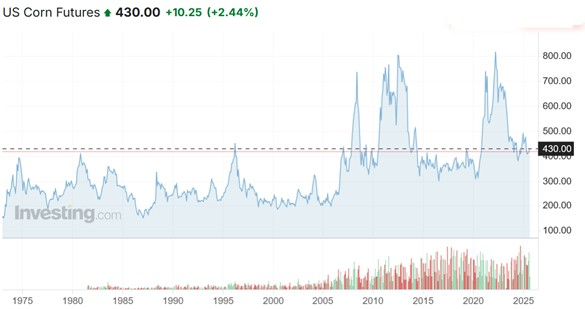
\includegraphics[width=0.5\textwidth]{figures/corn.jpg}
\end{center}

Mexico is structurally short yellow corn and imports most of it from the U.S., while white corn is central for tortillas. Policy has been in flux: Mexico's 2023 decree targeted biotech corn for human consumption and instructed a gradual substitution in other uses, triggering a USMCA dispute \citep{fas_mexico_decree_2023,ustr_usmca_biotech_2023}. In December 2024 the US prevailed at the USMCA panel \citep{ustr_usmca_biotech_win_2024}; Mexico has kept a domestic planting ban while adjusting import measures \citep{reuters_mexico_gm_ban_2025,fas_mexico_grain_annual_2025}. These shifts, together with U.S. supply and logistics, transmit into Mexican basis, feed costs, and tortilla inflation dynamics.

ZCZ5 denotes the CBOT Corn futures contract for December 2025 delivery (month code Z). Each contract is 5{,}000 bushels; tick size is $1/4$ cent per bushel (\$12.50 per contract) \citep{barchart_zc_specs}.
Recent U.S. balance-sheet news also matters: USDA has projected very large 2025 U.S. corn production, which weighs on deferred contracts like ZCZ5, all else equal \citep{reuters_record_crop_2025}.
% (Optional) Add a footnote if you want month codes spelled out.
\footnote{CBOT month codes: H=Mar, K=May, N=Jul, U=Sep, Z=Dec \citep{barchart_zc_specs}.}

\subsection{Pricing the ZCZ5 contract}
\begin{center}
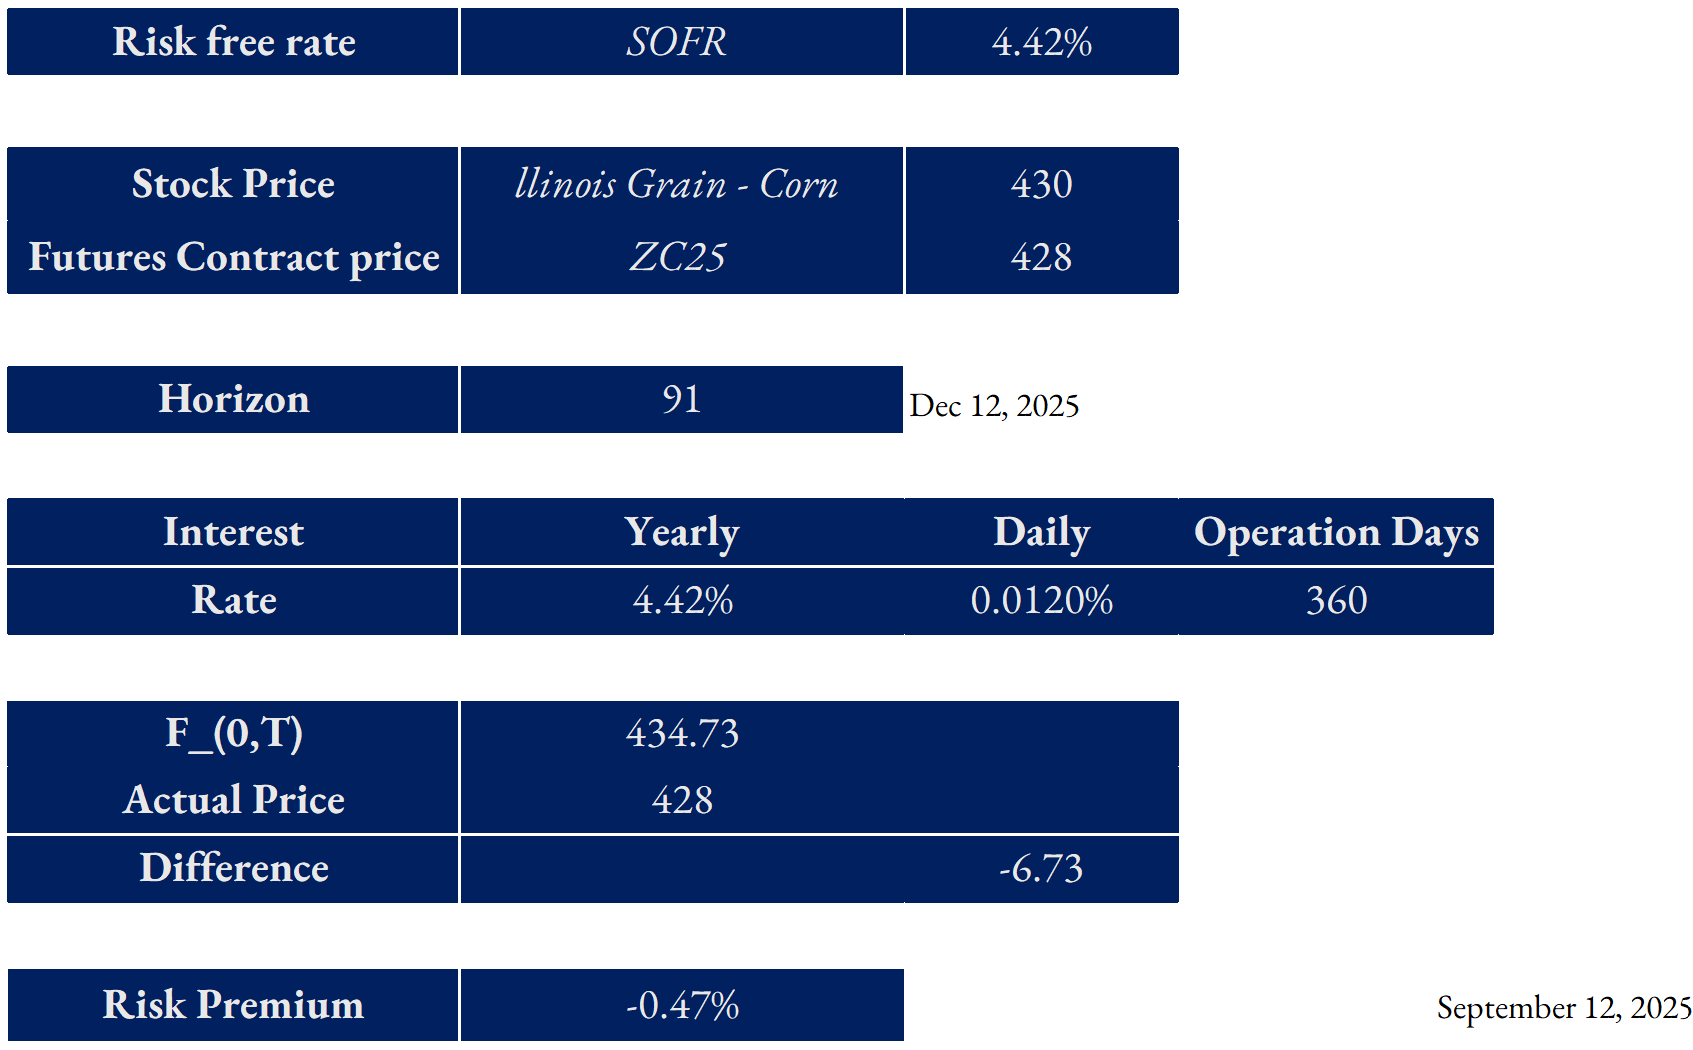
\includegraphics[width=0.5\textwidth]{figures/corn2.png}
\end{center}

A 91-day horizon (ACT/360) is used with $S=430.00$ ¢/bu for Illinois cash corn, $F=428.00$ ¢/bu for \textbf{ZCZ5}, and $r=4.41\%$. The no-carry fair value is obtained from $F^{\*}=S\,e^{rT}$, yielding
\[
T=\tfrac{91}{360},\quad F^{\*}=430\,e^{0.0441\cdot T}\approx \mathbf{434.72}\ \text{¢/bu}.
\]

A price difference of $\mathbf{-6.72}$ ¢/bu is observed $(F-F^{\*})$, which equals \textbf{26.9 ticks} and \textbf{\$336 per 5,000-bu contract}. The spot–futures return $F/S-1$ is $\mathbf{-0.47\%}$.

For interpretation, the cost-of-carry relation
\[
F=S\,e^{(r+u-y)T}
\]
is used, where $u$ represents storage and insurance costs and $y$ the convenience (or inventory) yield. The market carry is inferred as
\[
c_{\text{mkt}}=\frac{1}{T}\ln\!\frac{F}{S}
=\frac{1}{91/360}\ln\!\frac{428}{430}\approx \mathbf{-1.84\%}\ \text{per year}.
\]

It follows that the net convenience yield is obtained as
\[
y-u \approx r-c_{\text{mkt}}\approx 4.41\%-(-1.84\%)=\mathbf{6.25\%}\ \text{per year}.
\]

Therefore, a \textbf{negative basis} and $F<S e^{rT}$ are consistent with \textbf{backwardation}: near-dated corn is priced below pure financing carry because inventory availability, storage constraints, or location basis premia raise the value of holding physical grain now. The deviation is explained by $y$ and operational frictions, so it is interpreted as an inventory/logistics signal rather than a tradable arbitrage.


\section{Crude Oil}
Crude oil is one of the most important energy commodities, powering transportation, industry, and heating. Therefore, its price is influenced by a complex array of factors. One of the most significant is the balance between global supply and demand. During periods of strong economic growth, demand for oil increases due to higher transportation and manufacturing activity. Conversely, economic recessions can lead to a sharp drop in demand and lower prices \citep{eia_prices_2023}.

The decisions made by the Organization of the Petroleum Exporting Countries (OPEC) and its allies (OPEC+) are also a primary influence on oil prices. This group coordinates production levels among major oil-exporting nations. By restricting or increasing output, they can directly tighten or loosen global supply to stabilize or manipulate the market \citep{eia_opec_2024}.

Geopolitical events are a major source of price volatility. Conflicts, sanctions, or political instability in key oil-producing regions (like the Middle East, Russia, or Venezuela) can disrupt supply chains and threaten actual production, leading to fears of a shortage and spiking prices \citep{eia_prices_2023}.

Furthermore, fluctuations in the U.S. dollar significantly affect oil prices. Since oil is globally traded in U.S. dollars, a stronger dollar makes oil more expensive for countries using other currencies, which can dampen demand. A weaker dollar makes oil cheaper on international markets, potentially boosting demand \citep{bis_usd_commodity_2023,ecb_oil_usd_2024}.

In 2008, crude oil prices reached a historic peak. That July, the price of West Texas Intermediate (WTI) crude oil futures hit an all-time nominal high of \$147.27 per barrel. This surge was driven by a combination of robust global demand, geopolitical tensions, and significant financial speculation. From the start of 2007 to this peak, the price had increased by over 200\%. The subsequent crash later that year, as the global financial crisis crushed demand, demonstrates the extreme volatility of the oil market \citep{reuters_oil_peak_2008,worldbank_oil_spike_2008}.

\textbf{CLV25} refers to the WTI (West Texas Intermediate) crude oil futures contract that expires in October 2025. Each contract represents 1{,}000 barrels and is quoted in U.S. dollars (USD) per barrel \citep{cme_cl_specs,cme_cl_calendar}.
This table compares the spot price, \$62.69, with what the futures price “should” be over 10 days using the 4.41\% annual risk-free rate and assuming there are no extra costs/benefits such as dividends \citep{frbny_sofr}.

\begin{center}
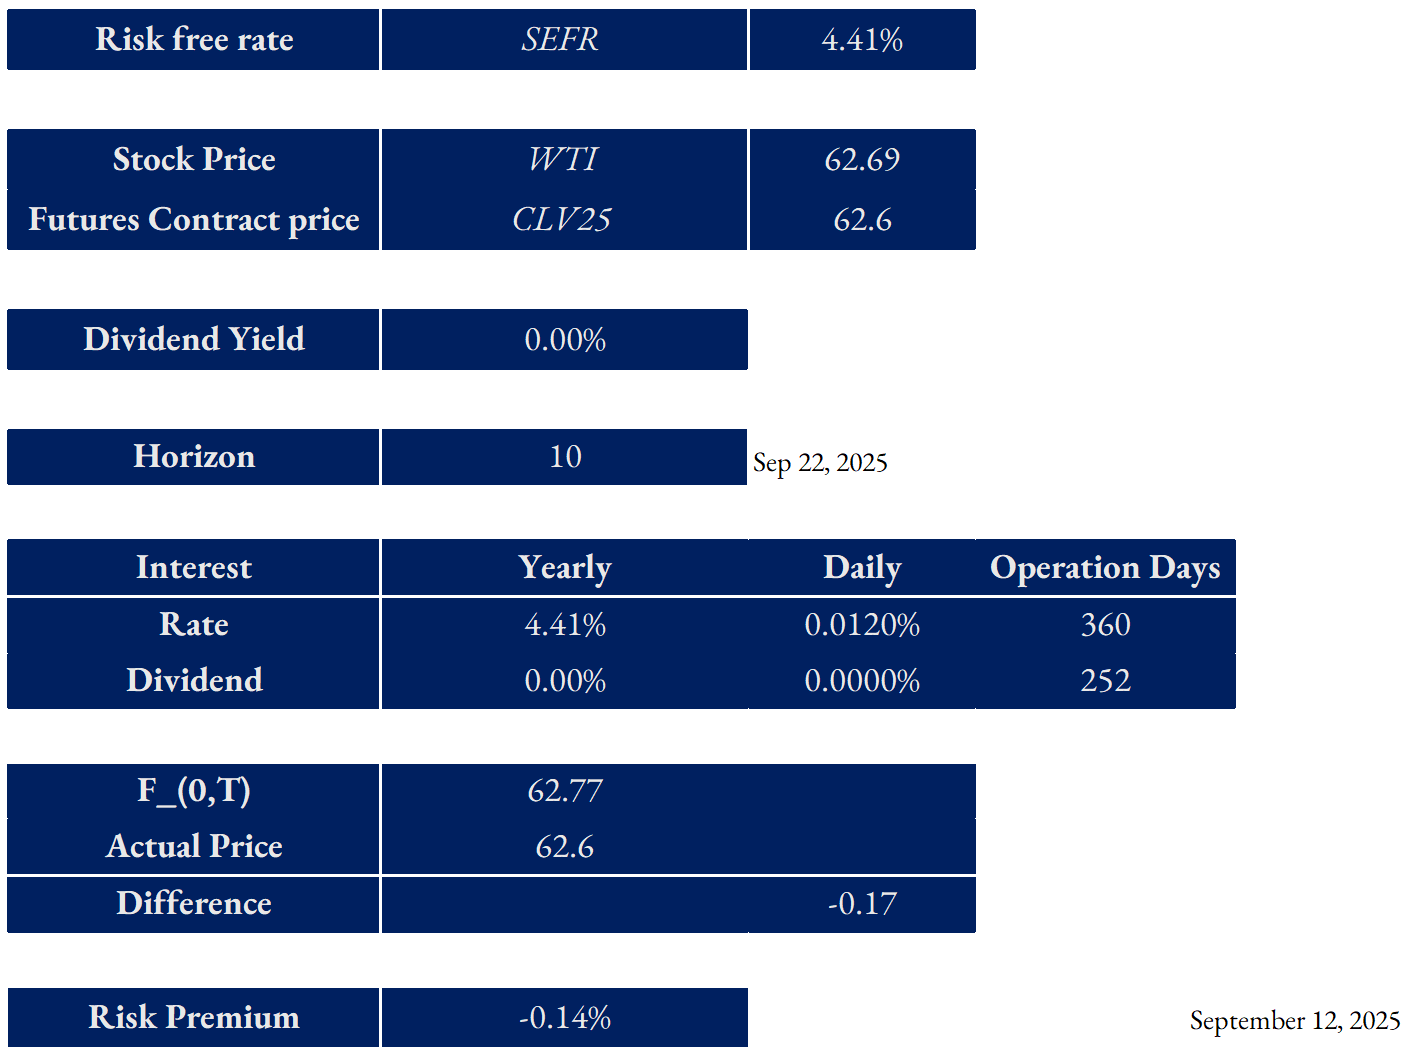
\includegraphics[width=0.5\textwidth]{figures/wti.png}
\end{center}

With those inputs, the theoretical price is computed as $F_{0,T} \approx S_0(1 + rT)$. For 10 days, $rT \approx 0.0441 \times \frac{10}{360} = 0.1225\%$. Therefore, $F_{0,T} \approx 62.69 \times (1 + 0.001225) = 62.77$. The market, however, is at 62.60. That means the actual futures price is \$0.17 per barrel below the theoretical value.

In percentage terms, the “risk premium” shown in the table is $-0.14\%$. That comes from comparing the futures price to spot: $62.60/62.69 - 1 \approx -0.14\%$. By contrast, the $-\$0.17$ difference you highlight is the gap between the market futures price and the theoretical futures price.

Economically, this discount indicates mild backwardation: the nearby contract is worth slightly less than what the interest rate alone would imply. In commodities like crude oil, this is often interpreted as an implicit convenience yield (the benefit of holding the physical now) that offsets the interest rate \citep{kaldor_working_brennan, eia_backwardation_2013, milonas_convenience_2024}. Roughly, the total deviation from the theoretical value is $\sim 0.2625\%$ over 10 days, which annualizes to about a $9.5\%$ convenience yield net of costs.

Practically speaking, for the standard contract size (1{,}000 barrels), that \$0.17 amounts to \$170 per contract \citep{cme_cl_specs}.


A 10-day valuation window is used with $S=62.69$, $F=62.60$, and $r=4.41\%$ (ACT/360). The no-carry fair value is computed as
\[
F^{\*}=S\,e^{rT}=62.69\,e^{0.0441\cdot(10/360)}\approx62.77.
\]

A price difference of
\[
-\$0.17
\]
per barrel is observed $(F-F^{\*})$, which corresponds to 17 ticks (\$170 per standard 1,000-barrel contract). In percentage terms, a spot–futures discount of
\[
\frac{F}{S}-1 \approx -0.14\%
\]
is obtained.

For interpretation, the cost-of-carry relation
\[
F=S\,e^{(r+u-y)T}
\]
is used, where $u$ denotes storage/insurance costs and $y$ denotes the convenience yield. The market carry is inferred as
\[
c_{\text{mkt}}=\frac{1}{T}\ln\!\frac{F}{S}\approx-5.17\%\ \text{per year},
\]
and the net convenience yield is obtained as
\[
y-u \approx r-c_{\text{mkt}}\approx 4.41\%-(-5.17\%)=9.6\% \ \text{per year}.
\]

Hence, the observed discount is consistent with \textbf{backwardation}: inventory is valued sufficiently highly (or storage is constrained) so that $y$ more than offsets financing $r$ and any $u$. No-arbitrage is preserved because $y$ and operational frictions are not directly tradable; the deviation is therefore read as a signal of tight near-term balances rather than a free arbitrage.



\section{Silver}
Silver has many uses, mainly in the industrial side. Therefore, there are many factors that influence its price. One of them is the global economy. Fluctuations in global growth or changes in monetary policies can impact demand for silver. Usually, during economic expansions, the demand for silver increases because of more manufacturing and technology. Fluctuations in currency can also affect demand for silver, especially talking about the US dollar. When the currency is stronger, the demand for silver is less because it is more expensive \citep{silver_institute_wss_2024,usgs_silver_mcs_2024,bis_usd_commodity_2023}.

\begin{figure}[h]
\centering
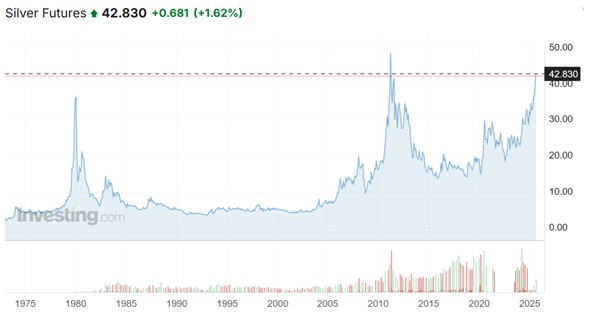
\includegraphics[width=0.7\textwidth]{figures/silver_time_series.jpg}
\caption{Silver futures price series. Source: Investing.com.}
\end{figure}

\paragraph{Geopolitical events are also an influence on silver prices.} Trade policies, tariffs, or tensions between nations can affect the supply chains and international trade that impact its availability and price \citep{silver_institute_wss_2024}.

\paragraph{In 1980 there was a big high in silver futures.} That event is known as Silver Thursday, and it referred to the Thursday 27th of March 1980 \citep{britannica_silver_thursday,nyt_1980_silver_thursday}.
On that day, the price of silver futures on the COMEX market in New York plummeted dramatically. The price had reached an all-time high of \$49.45 per ounce in January 1980, driven by a speculative frenzy largely fueled by the Hunt brothers, who attempted to corner the silver market. However, regulatory changes and margin calls led to a rapid collapse in prices, causing significant financial losses for many investors and leading to a broader market panic \citep{britannica_silver_thursday,nyt_1980_silver_thursday}.

\subsection{Recent developments}
Spot silver has breached multi-year highs in early September 2025, trading above \$40/oz and printing fresh 14-year peaks as U.S. rate-cut probabilities increased and the dollar softened; momentum has been reinforced by analyst upgrades that cite ETF inflows and a persistent physical deficit \citep{reuters_silver_14y_sep1,reuters_tradingday_sep11,reuters_anz_raises_silver,lbma_q2_2025}. Corporate activity remains supportive for Mexico-centric supply, with a pending acquisition that consolidates interest in the Juanicipio asset \citep{reuters_paasmag}. Benchmarking for spot valuation continues to rely on the LBMA Silver Price, while COMEX futures provide standardized hedging and exposure along the curve \citep{lbma_prices,cme_silver_overview}.

\paragraph{Mexico: why it matters.}
Mexico is the world’s leading silver producer; mining income, royalties, and FX earnings are sensitive to silver’s level and volatility \citep{reuters_mx_top_silver}. Higher prices improve cash flow and capex flexibility for domestic producers and their suppliers, while policy or logistics shocks can widen local basis. Stronger silver also interacts with MXN through the trade channel and risk sentiment: improved mining terms of trade are peso-supportive conditional on broader macro conditions.

\paragraph{spot vs.\ futures.}
The spot price of unallocated silver in London (or a deliverable loco), typically proxied by the LBMA Silver Price or XAG/USD spot quotes; it is used to value immediate physical transactions and inventory. By contrast, COMEX silver futures embed financing and inventory economics over a horizon \(T\). A standard cost-of-carry relation is used:
\[
F = S\,e^{(r+u-l)\,T},
\]
where \(r\) is the dollar funding rate, \(u\) represents storage/insurance, and \(l\) is the lease (or convenience) rate. When tightening in nearby physical markets raises \(l\) above \(r+u\), backwardation is obtained \((F<S\,e^{rT})\); when financing and storage dominate, contango is obtained. During episodes of rapid spot appreciation catalyzed by Fed-easing expectations and robust investor demand, it is common that lease rates rise and spot premia widen, so the futures curve can richen less than spot or even invert at the front. For Mexico-based producers, this distinction shapes hedge design: spot strength is used to lock revenue, while curve shape determines carry costs and roll outcomes on futures hedges.

\paragraph{Implications for Mexico-linked exposures.}
Given elevated spot levels and persistent tightness signals, it is expected that: (i) producers with near-term shipments benefit first via realized spot, (ii) longer-dated cash flows depend on curve structure and hedge discipline, and (iii) MXN correlations remain regime-dependent—improving terms of trade are supportive, but U.S. rate surprises and global risk cycles dominate at high frequency. Policy and permitting news can modulate this transmission, affecting local basis and project timing even when global prices are strong.


\subsection{Interpretation of SIZ25.}
A \textbf{positive basis} is observed: $F=42.83>F^{*}=42.74$, a premium of \textbf{\$0.09/oz} (18 ticks, \textbf{\$450} per 5,000-oz contract). With $S=42.195$ and a 108-day horizon $(T=108/360=0.30)$, the market carry is obtained as
\[
c_{\mathrm{mkt}} = \frac{1}{T}\ln\!\frac{F}{S}
= \frac{1}{0.30}\ln\!\frac{42.83}{42.195}
\approx \mathbf{4.97\%}\ \text{per year}.
\]

\begin{figure}[h]
\centering
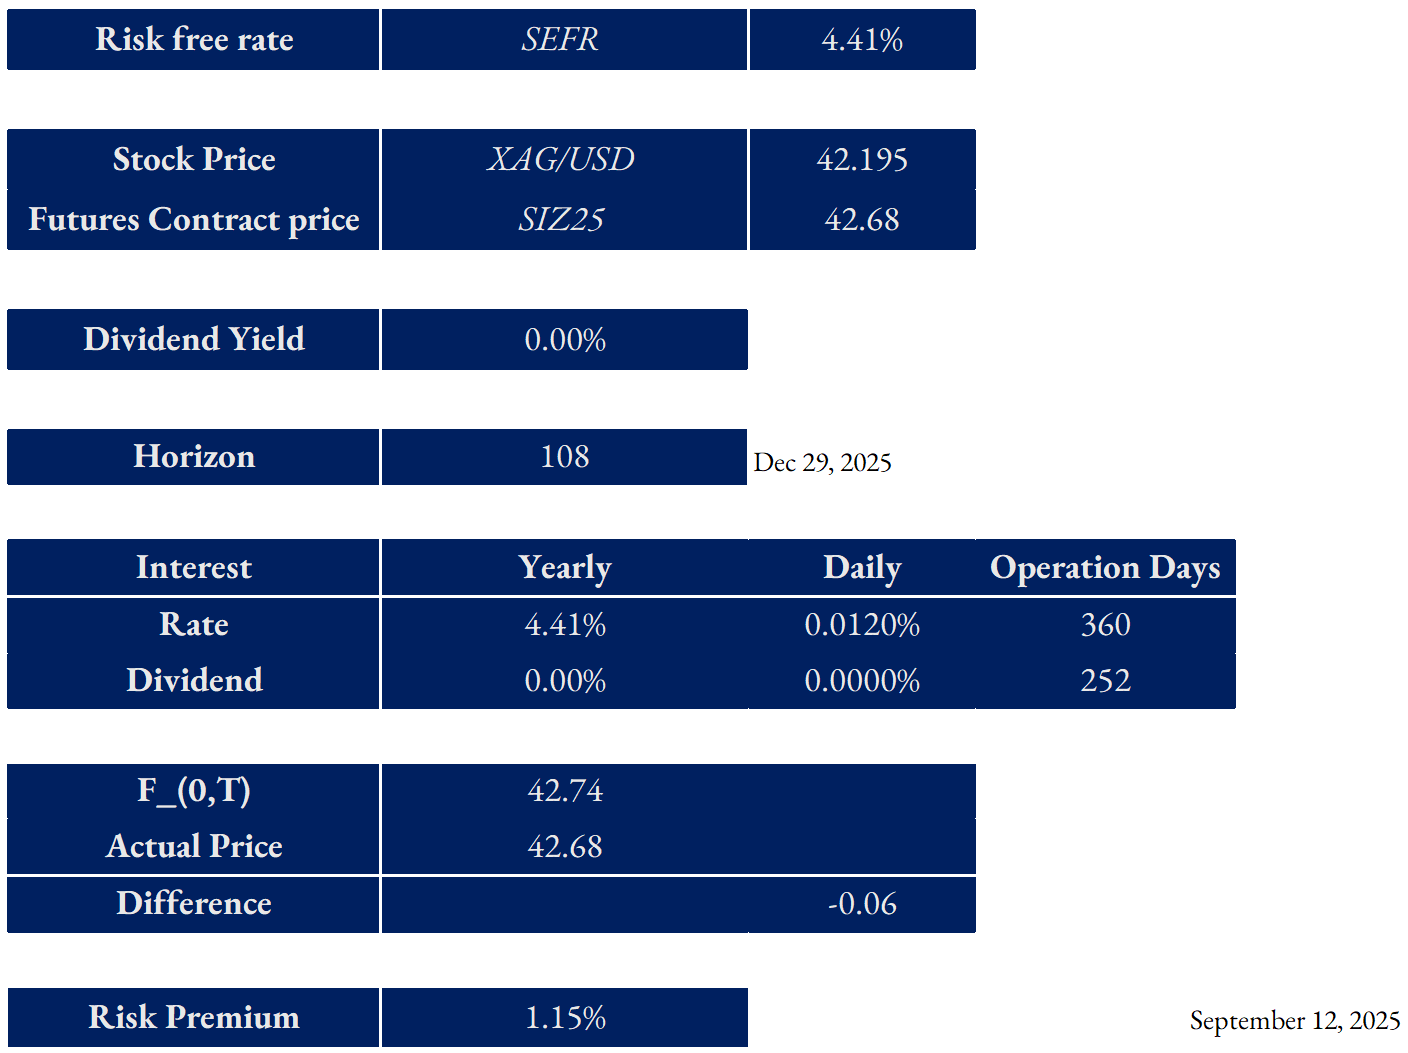
\includegraphics[width=0.7\textwidth]{figures/silver_pricing_one_day.png}
\caption{Pricing of SIZ25}
\end{figure}

Compared with the funding rate $r=4.41\%$, the implied \textbf{net storage minus lease rate} is
\[
u-l = c_{\mathrm{mkt}} - r \approx \mathbf{0.6\%}\ \text{per year},
\]
which is consistent with \textbf{contango}: financing and storage slightly exceed the lease (convenience) rate, so the futures price sits modestly above both spot $(F>S)$ and the pure-financing benchmark $(F>F^{*}=S e^{rT})$.

\paragraph{Why this aligns with the news.} Recent silver headlines emphasize multi-year highs driven by rising Fed-cut probabilities, a softer USD, ETF inflows, and talk of persistent physical deficits. Those forces primarily elevate the \textbf{spot} (the subyacente). However, the \textbf{futures} price capitalizes financing and inventory economics over the 108-day horizon. The observed, small premium indicates that—despite strong spot demand—the lease rate has \textbf{not} risen enough to overwhelm storage and funding costs. Adequate deliverable inventories, available storage, year-end financing effects, and investor preference to hold exposure via futures rather than immediate physical settlement are sufficient to keep the front of the curve in \textbf{slight contango}. The deviation is economically modest and should be read as a carry/liquidity effect rather than as a dislocation.

\subsection{Weekly read (cost-of-carry lens).}
Across 5--12 Sep 2025 the silver curve transitions from \textbf{mild backwardation} to \textbf{mild contango}. Early in the week, \textbf{Market $-$ Theoretical} is negative ($-\$0.02$ to $-\$0.11$/oz), which is consistent with a lease/convenience rate that temporarily \textbf{exceeds} financing plus storage; by Thu--Fri the sign flips positive ($+\$0.02$ to $+\$0.09$/oz), indicating that \textbf{financing and storage dominate} the lease rate over the remaining horizon. This evolution is consistent with the news backdrop: spot strength driven by rising Fed-cut odds and USD softness elevates the subyacente, while futures pricing incorporates funding and inventory economics; as immediate tightness eases or as futures demand is used for exposure, the front of the curve reverts to slight contango.

\begin{figure}[h]
\centering
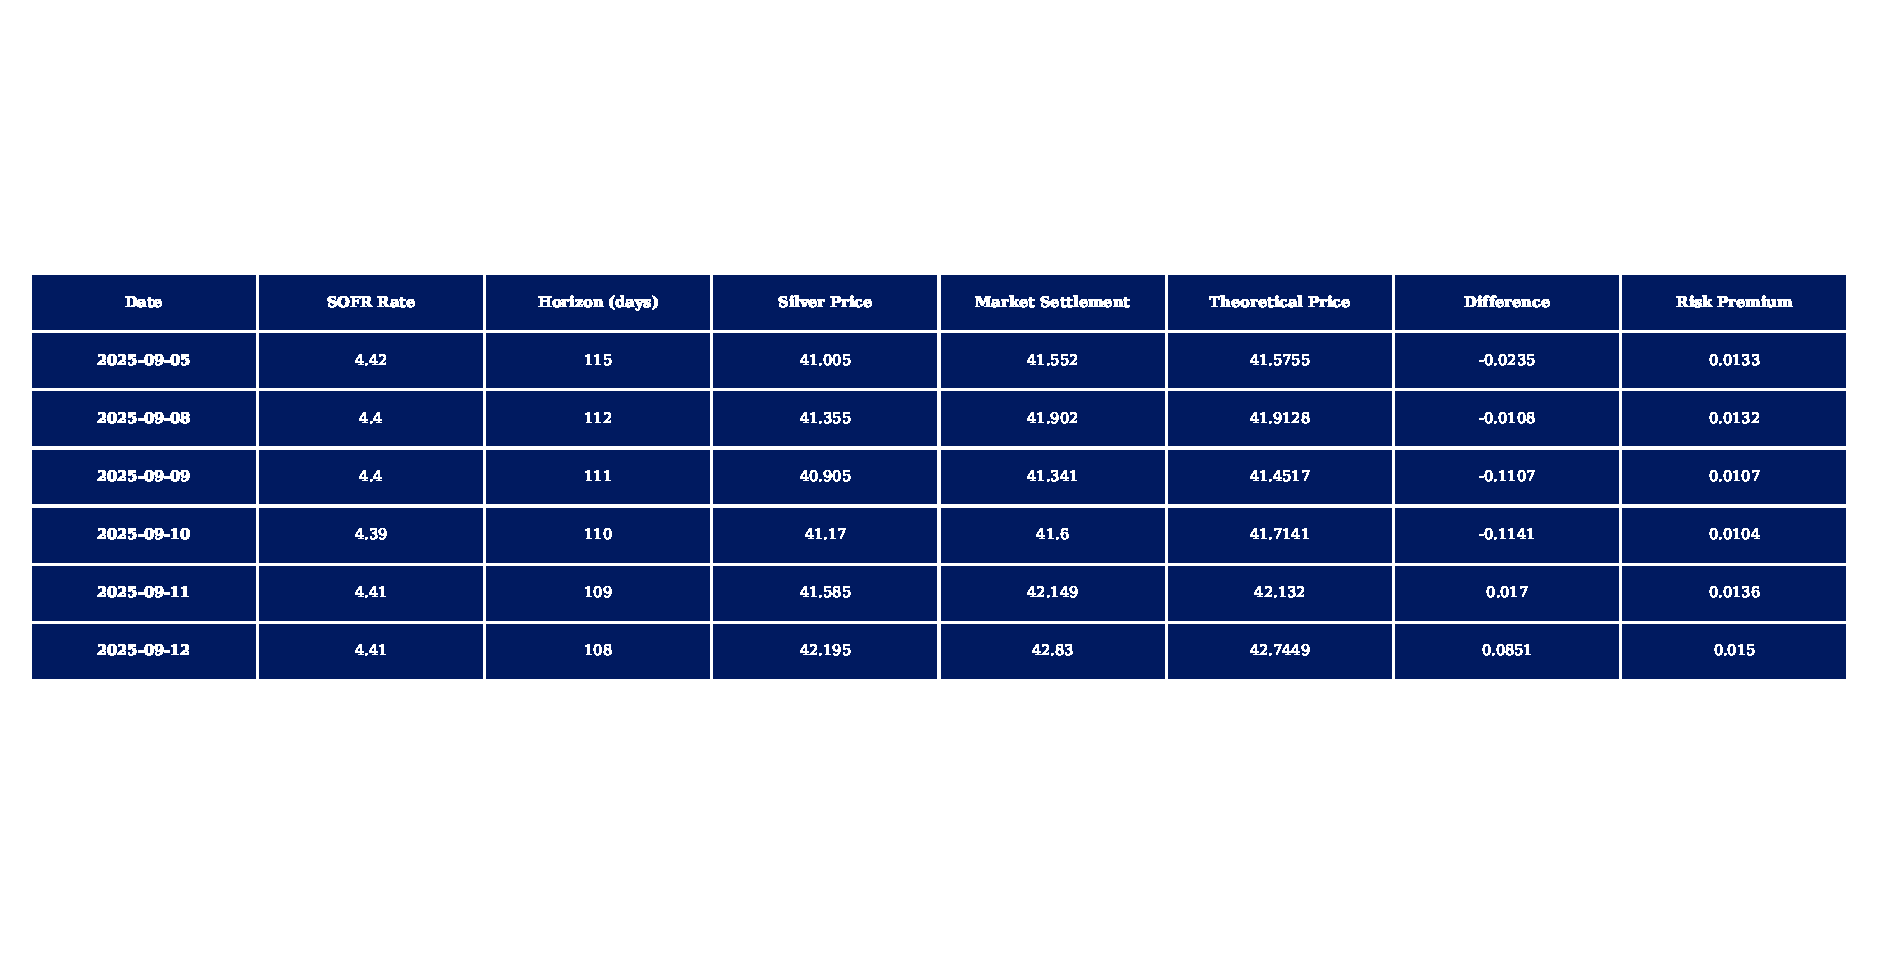
\includegraphics[width=1\textwidth]{figures/silver_pricing_over_the_week.pdf}
\caption{Pricing of SIZ25 over the week}
\end{figure}

\paragraph{Day-by-day classification and implied net carry.}
Using $F=S\,e^{(r+u-l)T}$ and $F^{\*}=S\,e^{rT}$, the net $u-l$ is obtained from $u-l=\tfrac{1}{T}\ln(F/F^{\*})$ (ACT/360; $T$ decreases from $\sim0.319$ to $\sim0.300$ over the week):

\begin{figure}[h]
\centering
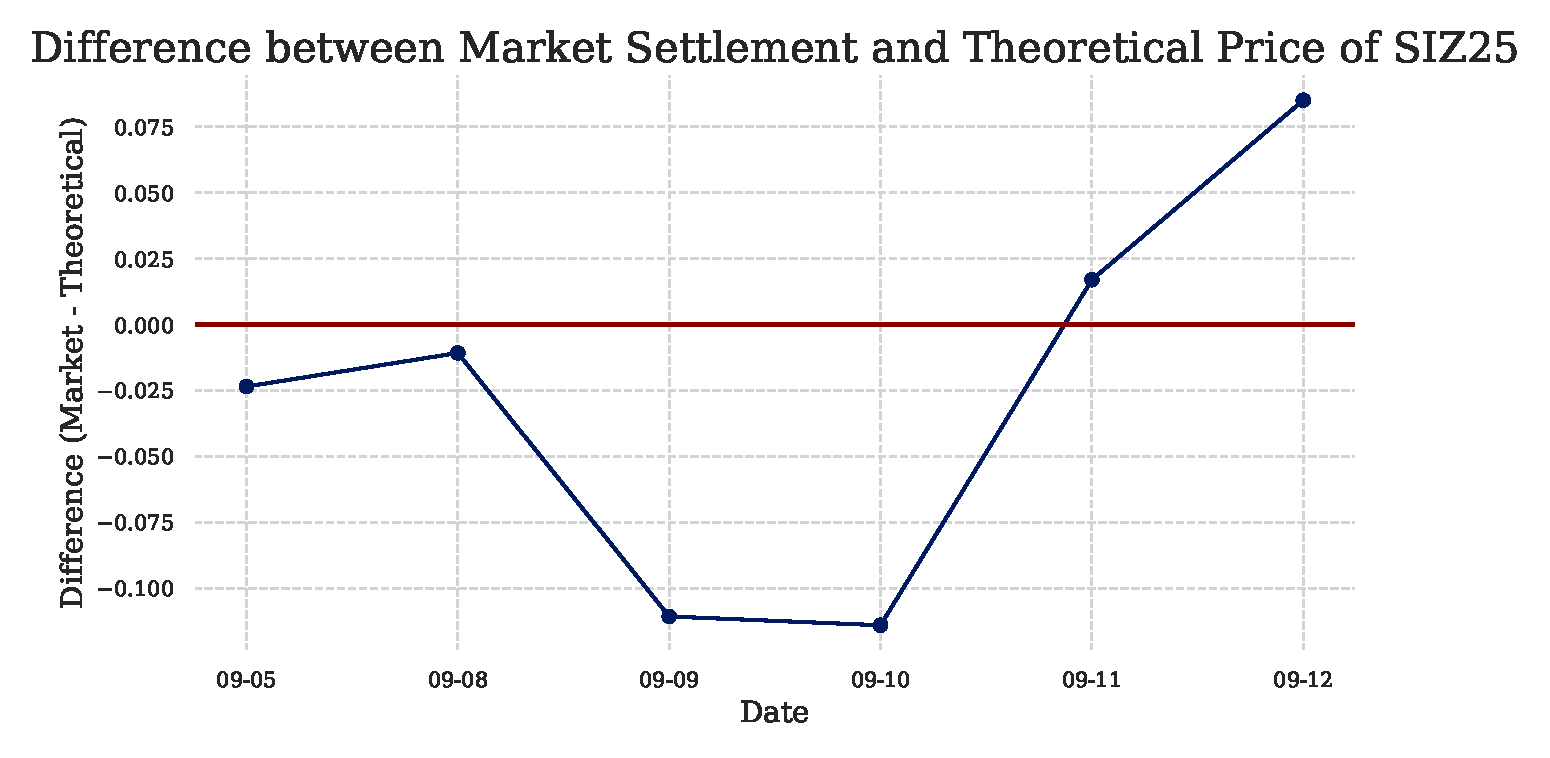
\includegraphics[width=0.7\textwidth]{figures/silver_difference.pdf}
\caption{Silver price series. Source: Investing.com.}
\end{figure}

\begin{itemize}
  \item \textbf{Fri 9/5:} $F-F^{*} = -\$0.024$ $\rightarrow$ \textbf{backwardation}; $u-l \approx -0.18\%$ p.a.
  \item \textbf{Mon 9/8:} $F-F^{*} = -\$0.011$ $\rightarrow$ \textbf{backwardation}; $u-l \approx -0.08\%$ p.a.
  \item \textbf{Tue 9/9:} $F-F^{*} = -\$0.111$ $\rightarrow$ \textbf{backwardation}; $u-l \approx -0.87\%$ p.a.
  \item \textbf{Wed 9/10:} $F-F^{*} = -\$0.114$ $\rightarrow$ \textbf{backwardation}; $u-l \approx -0.89\%$ p.a.
  \item \textbf{Thu 9/11:} $F-F^{*} = +\$0.017$ $\rightarrow$ \textbf{contango}; $u-l \approx +0.13\%$ p.a.
  \item \textbf{Fri 9/12:} $F-F^{*} = +\$0.085$ $\rightarrow$ \textbf{contango}; $u-l \approx +0.66\%$ p.a.
\end{itemize}

\begin{figure}[h]
\centering
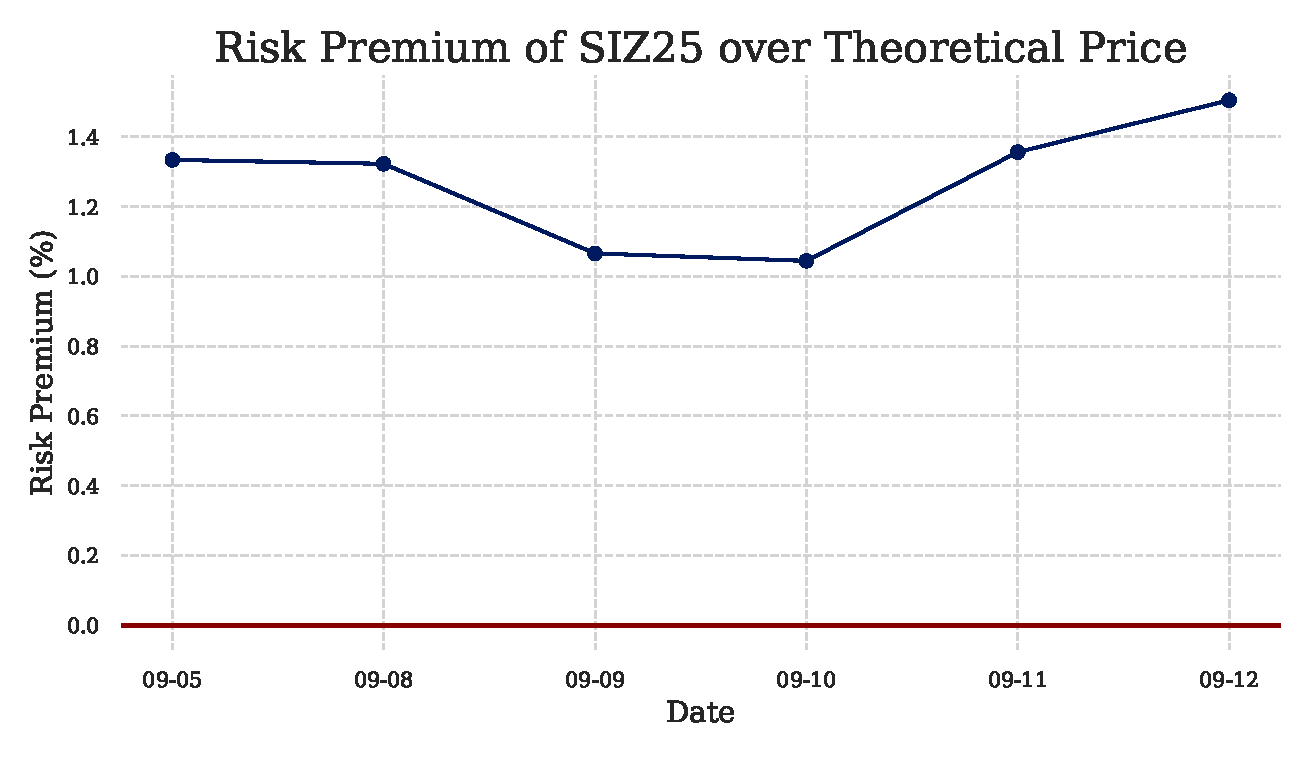
\includegraphics[width=0.7\textwidth]{figures/silver_risk_premium.pdf}
\caption{Silver price series. Source: Investing.com.}
\end{figure}

\paragraph{Forward premium vs.\ spot.}
The ``Risk Premium'' column $(F/S-1)$ stays small ($\approx 1.06$--$1.50\%$). It dips mid-week as spot outperforms, then rises as futures regain a modest premium. Economically, this forward premium is used to summarize \textbf{carry} (funding $+$ storage $-$ lease). It should be interpreted as a carry/liquidity effect, not as an arbitrage.


\section{Silver}

In this section, the economic role, policy drivers, historical stress episode, recent developments, spot versus futures framework, and Mexico-linked implications of silver are discussed.

\subsection{Economic role and macro-financial channels}
Silver is a dual-use metal with a large industrial footprint (electronics, photovoltaics, medical and chemical applications) and a non-trivial investment component. As a result, its pricing is shaped by both end-use demand and financial conditions. Cyclical expansions raise manufacturing throughput and technology adoption, lifting physical offtake; global slowdowns reverse that impulse. Monetary policy and term premia transmit through discount rates and the USD: a stronger dollar tightens global financial conditions and lowers non-USD purchasing power, dampening demand for dollar-priced commodities; a softer USD does the opposite \citep{silver_institute_wss_2024,usgs_silver_mcs_2024,bis_usd_commodity_2023}.

\begin{figure}[h]
\centering
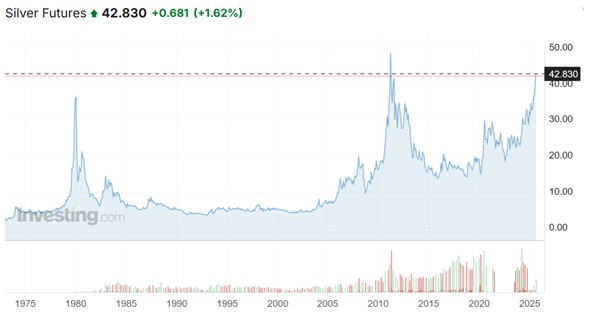
\includegraphics[width=0.7\textwidth]{figures/silver_time_series.jpg}
\caption{COMEX silver futures time series (illustrative). Source: Investing.com.}
\label{fig:silver_time_series}
\end{figure}

\subsection{Policy and geopolitical drivers}
Trade restrictions, tariffs, sanctions, and logistics frictions reallocate flows across refining hubs and end-user markets, altering local basis and inventory dynamics; these mechanisms operate alongside the macro channels above \citep{silver_institute_wss_2024}.

\subsection{Historical stress episode}
The 1980 episode (“Silver Thursday”) illustrates how leverage, concentrated positioning, and margining can dominate price discovery. After a speculative run-up to \$49.45/oz, rule changes and margin calls precipitated a sharp decline on March 27, 1980, with broader market spillovers \citep{britannica_silver_thursday,nyt_1980_silver_thursday}.

\subsection{Recent developments}
In early September 2025, spot silver traded above \$40/oz and marked 14-year highs amid rising Fed-easing probabilities and a weaker USD; research commentary highlighted ETF inflows and a persistent physical deficit \citep{reuters_silver_14y_sep1,reuters_tradingday_sep11,reuters_anz_raises_silver,lbma_q2_2025}. Corporate activity remains supportive for Mexico-centric supply, including consolidation around the Juanicipio asset \citep{reuters_paasmag}. Spot benchmarking relies on the LBMA Silver Price, while COMEX futures provide standardized exposure and hedging along the term structure \citep{lbma_prices,cme_silver_overview}.

\paragraph{Mexico: why it matters.}
Mexico is the world’s largest silver producer, so revenue, royalties, and FX inflows are sensitive to the level and volatility of silver. Higher prices improve internal cash generation and capex flexibility; conversely, regulatory or logistical frictions widen local basis and delay monetization. Through the terms-of-trade channel, stronger silver can be peso-supportive when broader macro conditions are aligned \citep{reuters_mx_top_silver}.

\subsection{Spot versus futures (interpretive framework)}
The spot price refers to unallocated silver in London (or a deliverable loco) and is used to value immediate transactions and inventories. COMEX futures internalize financing and inventory economics over horizon \(T\) via the cost-of-carry relation
\[
F=S\,e^{(r+u-l)T},
\]
with \(r\) the USD funding rate, \(u\) storage/insurance, and \(l\) the lease (convenience) rate. Tight nearby physical conditions raise \(l\) and can generate backwardation \((F<S\,e^{rT})\); abundant storage and higher financing tilt the curve toward contango. Thus, spot primarily reflects contemporaneous scarcity and dollar conditions, while futures reflect the intertemporal trade-off between owning inventory today versus financing delivery later.

The \emph{spot} benchmark is the LBMA Silver Price (or XAG/USD quotes for unallocated metal in London); it is used to value immediate physical transactions, inventory revaluation, and cash-market settlements \citep{lbma_prices}. The COMEX futures curve is used to transfer price risk across time and to standardize hedging and speculative exposure; contract design, margining, and delivery mechanics shape its microstructure \citep{cme_silver_overview}. In practice, three news-sensitive wedges separate spot from futures: (i) the \emph{financing–storage–lease} term in the cost-of-carry \(F=S\,e^{(r+u-l)T}\), (ii) \emph{location/quality} basis between London unallocated and COMEX-deliverable bars, and (iii) \emph{timing} basis linked to near-term ETF creations/redemptions and refinery/warehouse flows. When easing U.S. rate expectations strengthen non-USD demand and ETF creations accelerate, it is common that spot tightens faster than the curve (lease rate \(l\uparrow\)), generating transient backwardation; as inventories are replenished and funding/storage regain prominence, slight contango reappears. Hence, spot is used as a barometer of contemporaneous scarcity and USD conditions, whereas futures are used to price the intertemporal trade-off between carrying inventory and deferring settlement.

\subsection{Mexico-linked implications}
Near-term shipments monetize elevated spot first; medium-dated cash flows depend on the curve’s carry and roll costs. Hedge design should distinguish (i) price level risk (spot) from (ii) term-structure risk (roll yield and basis), recognizing that cross-currency and policy shocks can modulate both even when the global price is strong.

Mexico’s role as the world’s largest silver producer means that domestic cash flows, royalties, and FX receipts are highly exposed to these spot–futures dynamics \citep{reuters_mx_top_silver}. The following news-driven scenarios are operationally relevant:
\begin{enumerate}
  \item \textbf{ETF inflow surges and USD weakness.} Spot premia rise first; it is used by producers with near-term shipments to monetize higher LBMA realizations. If COMEX contango persists, rolling short futures hedges entails modest carry costs; if backwardation appears, rolls can be revenue-positive.
  \item \textbf{Refinery or logistics bottlenecks.} Delays in moving Mexico-origin doré or concentrates to refiners widen the location basis versus London. It is used to hedge with COMEX futures, but performance depends on the basis path; treasury policy should stress-test basis risk alongside price risk.
  \item \textbf{Funding-cost swings.} Shifts in dollar funding alter \(r\) and, with stable lease \(l\), move the curve even if spot is unchanged; this is used to reassess hedge tenors because forward premia/discounts change while realized sales prices do not.
  \item \textbf{Domestic policy shocks.} Changes in royalties, permitting, power tariffs, or labor conditions affect mining margins and supply timing; it is used to adjust production hedges and to reassess the mix of spot sales versus forward coverage given altered cash-need profiles.
  \item \textbf{FX interaction (USD/MXN).} Stronger silver improves Mexico’s terms of trade and can support MXN conditionally on global risk; however, a stronger MXN reduces peso revenues for unhedged USD sales. It is used to pair metal hedges with FX hedges to stabilize MXN cash flows.
\end{enumerate}
In summary, elevated spot levels benefit near-term Mexican exports directly, while the sign and size of the futures basis determine carry and roll outcomes on hedges. Policy- and logistics-sensitive basis risk is material; it is used to complement price hedging with explicit basis and FX risk management, recognizing that the curve reflects financing and inventory conditions that need not move one-for-one with spot.


\subsection{Interpretation of \texorpdfstring{SIZ25}{SIZ25} (one-day read)}
A \emph{positive basis} is observed: \(F=42.83>F^{*}=42.74\), a premium of \$0.09/oz (18 ticks, \$450 per 5{,}000-oz contract). With \(S=42.195\) and \(T=108/360\), the market carry is
\[
c_{\mathrm{mkt}}=\frac{1}{T}\ln\!\frac{F}{S}
=\frac{1}{0.30}\ln\!\frac{42.83}{42.195}\approx 4.97\%\ \text{p.a.}
\]
Relative to \(r=4.41\%\), the implied net storage minus lease is
\[
u-l=c_{\mathrm{mkt}}-r\approx 0.6\%\ \text{p.a.},
\]
consistent with \emph{slight contango}: financing plus storage marginally exceed the lease rate, so the future sits above spot and above the pure-financing benchmark \(F^{*}=S\,e^{rT}\). This aligns with contemporaneous news: strong demand and a softer USD lift spot, yet lease rates have not risen enough to overcome carry costs over 108 days.

\begin{figure}[h]
\centering
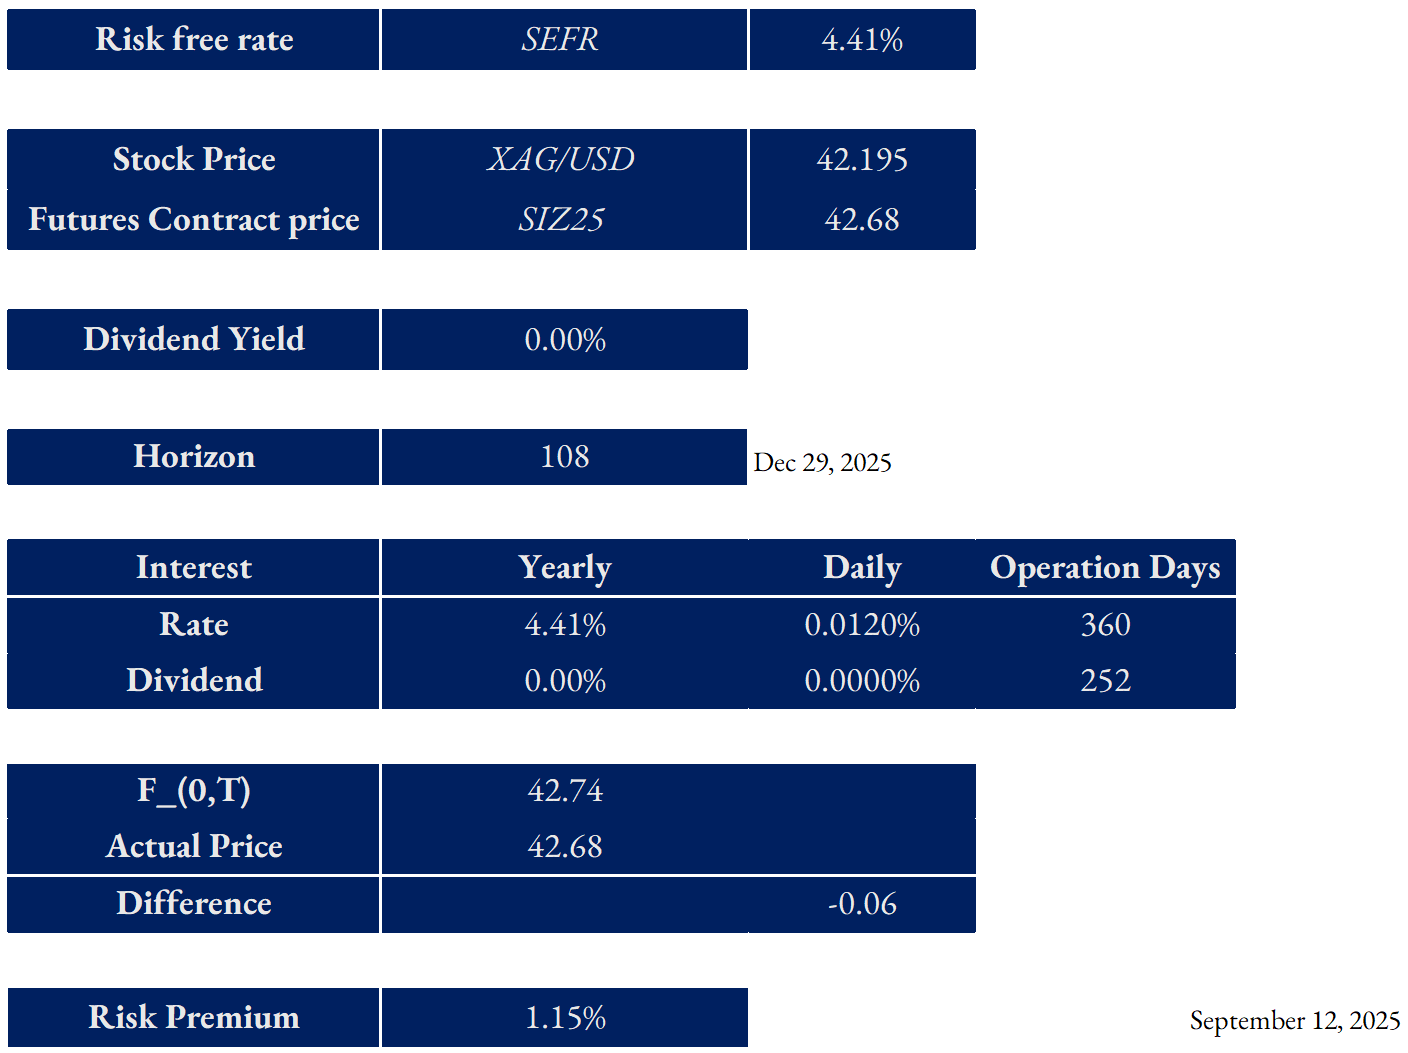
\includegraphics[width=0.7\textwidth]{figures/silver_pricing_one_day.png}
\caption{One-day pricing decomposition for SIZ25.}
\label{fig:silver_one_day}
\end{figure}


A small, but statistically meaningful, \emph{positive basis} is observed on \emph{September 12, 2025}: \(F=42.83>F^{*}=42.74\), i.e., a premium of \(\$0.09/\mathrm{oz}\) (18 ticks, \(\$450\) per 5{,}000-oz contract). With \(S=42.195\) and \(T=108/360\), the market-implied carry is
\[
c_{\mathrm{mkt}}=\frac{1}{T}\ln\!\frac{F}{S}=\frac{1}{0.30}\ln\!\frac{42.83}{42.195}\approx 4.97\% \ \text{p.a.}
\]
Given a funding benchmark \(r=4.41\%\), the net inventory term is obtained as
\[
u-l=c_{\mathrm{mkt}}-r\approx 0.60\%\ \text{p.a.}
\]
This decomposition is used to interpret the premium as \emph{slight contango}: financing and storage together exceed the lease (convenience) rate by a few basis points on an annualized basis, so the future prices above both spot and the pure-financing benchmark \(F^{*}=S\,e^{rT}\).

\begin{figure}[h]
\centering
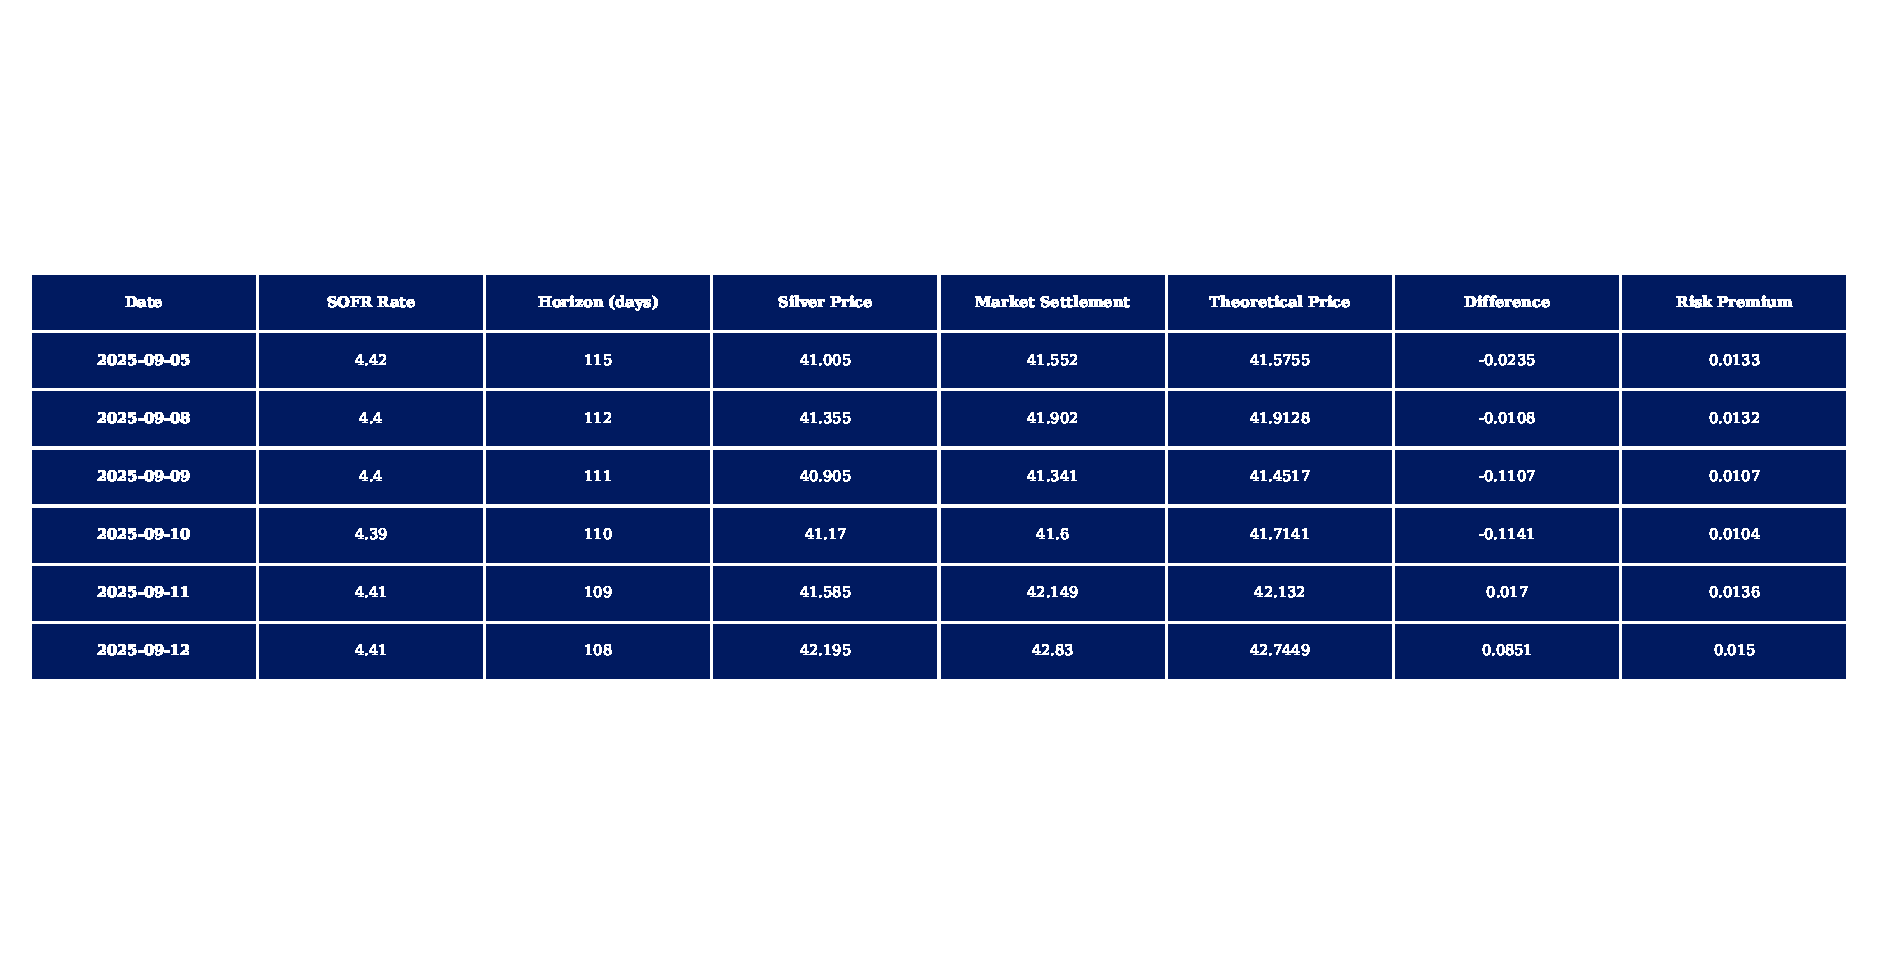
\includegraphics[width=\textwidth]{figures/silver_pricing_over_the_week.pdf}
\caption{Weekly evolution of Market \(-\) Theoretical and risk premium for SIZ25.}
\label{fig:silver_week}
\end{figure}


\paragraph{Why this is consistent with the news flow.}
Contemporaneous headlines emphasize (i) elevated spot levels on rising Fed-cut probabilities and a softer USD, (ii) ETF-related investor demand, and (iii) discussion of structural deficits. These elements are used to lift the \emph{subyacente} first; however, the futures price capitalizes financing and inventory over the next 108 days. The small, positive \(u-l\) indicates that, notwithstanding robust spot demand, lease rates have not surged enough to dominate funding and storage for this horizon. Adequate deliverable stocks, available storage, and year-end financing conditions can sustain a modest contango even as spot remains buoyant. Economically, this is read as a \emph{carry/liquidity configuration}, not as a dislocation or an arbitrage.


\begin{figure}[h]
\centering
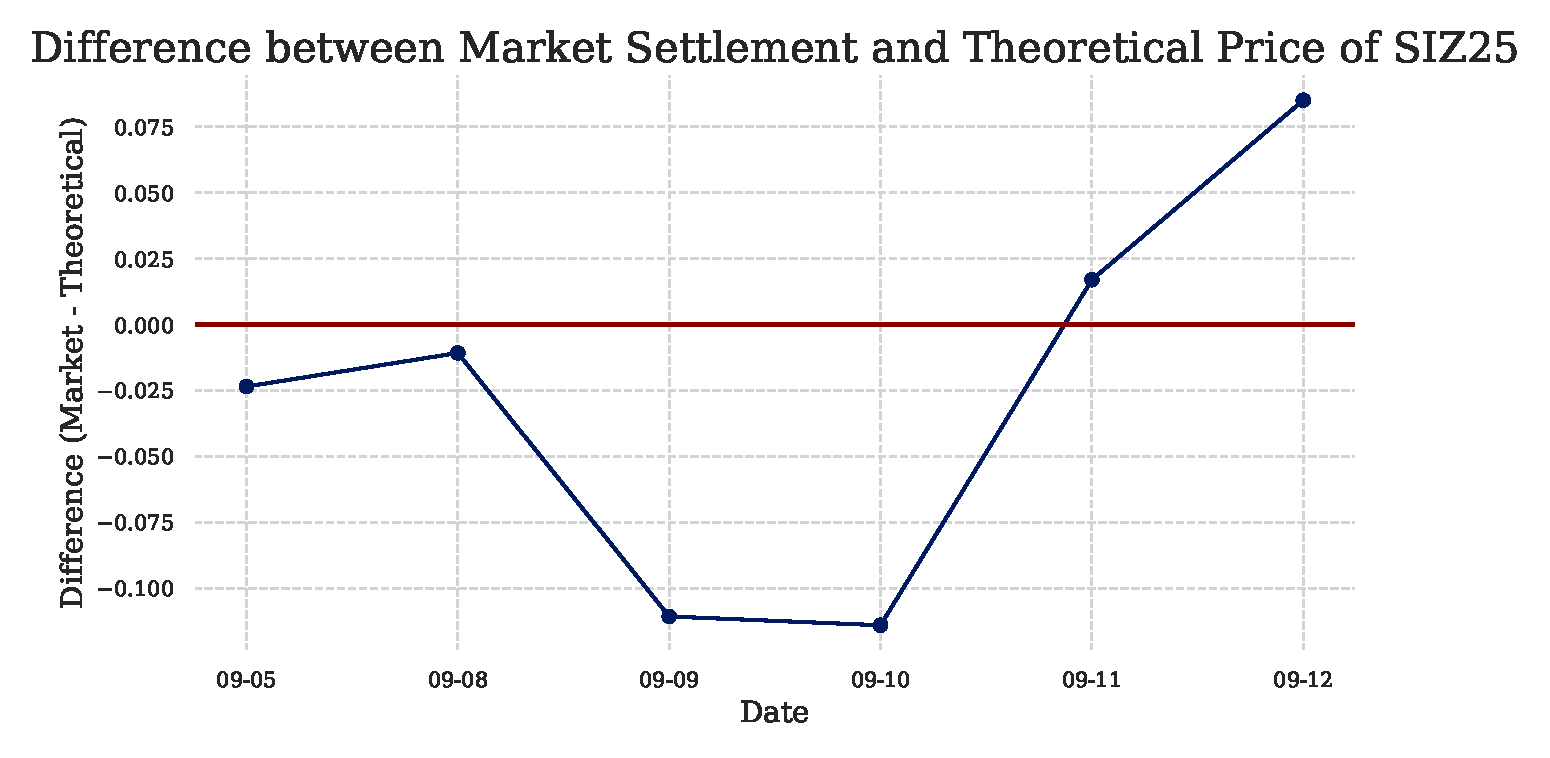
\includegraphics[width=0.7\textwidth]{figures/silver_difference.pdf}
\caption{Daily difference \(F-F^{*}\) and sign (backwardation vs.\ contango).}
\label{fig:silver_difference}
\end{figure}


\medskip
\noindent\emph{Risk classification.} The premium sits well within typical no-arbitrage bands once bid–ask, exchange fees, collateral haircuts, and delivery frictions are recognized. Positioning should therefore emphasize curve-shape risk (carry and roll) rather than seeking to monetize an illusory mispricing.


\subsection{Weekly term-structure diagnostics (5–12 Sep 2025)}
Table-based evidence indicates a transition from \emph{mild backwardation} early in the week (negative Market \(-\) Theoretical) to \emph{mild contango} by Thursday–Friday (positive spreads). Interpreting \(u-l=\tfrac{1}{T}\ln(F/F^{*})\) with ACT/360:
\begin{itemize}
  \item \textbf{9/5–9/10:} negative spreads (\(-\$0.02\) to \(-\$0.11\)/oz) imply \(l>r+u\): nearby inventory scarcity and/or elevated lease rates.
  \item \textbf{9/11–9/12:} positive spreads (\(+\$0.02\) to \(+\$0.09\)/oz) imply \(r+u>l\): easing tightness and/or stronger preference for futures exposure that capitalizes carry.
\end{itemize}
The “Risk Premium” \((F/S-1)\) remains small (≈1.06–1.50\%), dipping when spot outperforms and recovering as futures regain a modest premium. Economically, this premium summarizes carry (funding \(+\) storage \(-\) lease) and is best interpreted as a liquidity/carry effect rather than an arbitrage opportunity.


The term structure transitions from \emph{mild backwardation} to \emph{mild contango} over the week. Early readings (\(F-F^{*}<0\)) are used to infer \(l>r+u\) for short horizons—consistent with transient tightness or elevated borrow in the physical market—while late-week readings (\(F-F^{*}>0\)) indicate \(r+u>l\) as funding and storage reassert dominance.

\paragraph{Day-by-day interpretation.}
Using \(u-l=\frac{1}{T}\ln(F/F^{*})\) (ACT/360; \(T\) declines from \(\sim 0.319\) to \(\sim 0.300\)):
\begin{itemize}
  \item \textbf{Fri 9/5:} \(F-F^{*}=-\$0.024\) \(\Rightarrow\) mild backwardation; \(u-l\approx-0.18\%\) p.a. It is used to read near-term inventory value as slightly elevated relative to carry.
  \item \textbf{Mon 9/8:} \(F-F^{*}=-\$0.011\) \(\Rightarrow\) mild backwardation; \(u-l\approx-0.08\%\) p.a. Tightness signal weakens; curve moves toward flat.
  \item \textbf{Tue 9/9:} \(F-F^{*}=-\$0.111\) \(\Rightarrow\) backwardation; \(u-l\approx-0.87\%\) p.a. A sharper spot-led impulse is used to widen the lease premium.
  \item \textbf{Wed 9/10:} \(F-F^{*}=-\$0.114\) \(\Rightarrow\) backwardation; \(u-l\approx-0.89\%\) p.a. Persistence of tightness; curve remains inverted at the front.
  \item \textbf{Thu 9/11:} \(F-F^{*}=+\$0.017\) \(\Rightarrow\) slight contango; \(u-l\approx+0.13\%\) p.a. The balance shifts; funding/storage begin to dominate.
  \item \textbf{Fri 9/12:} \(F-F^{*}=+\$0.085\) \(\Rightarrow\) contango; \(u-l\approx+0.66\%\) p.a. A normalized carry regime is used to characterize the close of the week.
\end{itemize}

\paragraph{Mechanistic drivers behind the flip.}
Three operational channels are typically implicated: (i) \emph{funding}—a rise in Fed-cut odds lowers expected discount rates but can steepen near-term collateral demand, dynamically affecting \(r\) relative to \(l\); (ii) \emph{inventory/warehouse}—refinery and warehouse flows can replenish deliverables, compressing lease premia; (iii) \emph{term demand}—investors may prefer futures exposure to defer physical handling, lifting \(F\) relative to spot once the initial spot-led surge abates. The observed risk premium \((F/S-1\approx 1.06\% \text{ to } 1.50\%)\) remains small; it is used as a summary statistic of carry rather than a tradable edge.

\subsection{Does this benefit Mexico? What should be done?}

\paragraph{Economic incidence for Mexico.}
As the leading global producer, Mexico is positioned to benefit from elevated spot and orderly term structure. The one-day contango and the week’s re-steepening are used to indicate that (i) near-term shipments monetize high spot realizations, and (ii) forward coverage can be implemented with manageable roll costs. FX pass-through matters: stronger silver improves terms of trade and is often peso-supportive, yet a stronger MXN reduces peso-denominated revenues unless currency risk is hedged.

\paragraph{Implications for investors (policy-neutral).}
\begin{enumerate}
  \item \textbf{Separate spot risk from curve risk.} It is used to treat price level (\(S\)) and roll/carry (\(F-S\), shape) as distinct. Long spot exposure benefits from the current level; futures strategies should model carry explicitly.
  \item \textbf{Hedge design.} For producers and MXN-based portfolios, it is used to pair metal hedges with FX hedges to stabilize peso cash flows. With slight contango, rolling short COMEX futures entails modest carry costs; in backwardation windows, rolls may be revenue-positive.
  \item \textbf{Tenor selection.} It is used to choose hedge tenors where \(u-l\) is stable and liquidity is deep (e.g., front two contract months), minimizing basis and execution risk.
  \item \textbf{Basis management.} Location and quality basis between London unallocated and COMEX deliverable bars should be monitored; treasury policy is used to set limits on basis drift and to pre-approve alternative hedging venues if needed.
\end{enumerate}

\paragraph{Implications for Mexico (policy and operating environment).}
\begin{enumerate}
  \item \textbf{Logistics and permitting reliability.} It is used to prioritize predictable permitting timelines and logistics corridors; stable, transparent processes compress location basis and reduce lease-rate spikes tied to bottlenecks.
  \item \textbf{Energy and power reliability.} Processing and refining require stable power; reliability improvements lower effective storage/operating costs \(u\), improving net margins across the cycle.
  \item \textbf{Market infrastructure and risk management.} It is used to encourage the adoption of standardized hedge programs (including FX overlays) among medium-size producers to align with best practices and reduce macro-volatility transmission to local cash flows.
  \item \textbf{Tax and royalty neutrality to hedging.} It is used to ensure that fiscal rules treat realized hedge outcomes neutrally relative to spot sales, avoiding distortions that discourage prudent risk transfer.
\end{enumerate}

\medskip
\noindent\emph{Synthesis.} The current configuration—high spot with slight, later-week contango—supports Mexican revenues while keeping roll costs contained. For investors, it is used to favor disciplined hedge-and-carry implementations that respect term-structure signals. For policymakers, reducing operational frictions and basis volatility enhances the capacity to translate favorable global prices into stable domestic income and investment.








\section{MXN/USD}
The exchange rate of the Mexican Peso (MXN) against the US Dollar (USD) is a crucial indicator of the Mexican economy and is influenced by a complex mix of domestic and international factors. One of the most important is the monetary policy of the US Federal Reserve (Fed). When the Fed raises its interest rates, the dollar strengthens, attracting investment into dollar-denominated assets and commonly causing a depreciation of the peso (i.e., it takes more pesos to buy one dollar). Similarly, interest rate decisions by the Bank of Mexico (Banxico) impact the exchange rate; higher rates can strengthen the peso by attracting foreign investment \citep{dallasfed_peso_2023,banxico_regional_2024}.

The overall state of the worldwide economy and investors' willingness to engage in risk are also pivotal determinants. The MXN is considered a "risk currency" or an "emerging market currency." During periods of global optimism and stability, investors often seek higher returns in emerging markets like Mexico, which appreciates the peso. Conversely, in times of uncertainty, geopolitical tension, or global recessions, investors seek safe-haven assets like the US dollar, triggering a massive sell-off of pesos and its depreciation \citep{bis_eme_internationalisation_2022}.

Internal factors and Mexico's economic situation play a fundamental role. Macroeconomic data such as GDP growth, the unemployment rate, inflation, and consumer confidence affect the perception of the country's stability. Furthermore, political events like elections, changes in fiscal policy (budgets, taxes), or the implementation of structural reforms can generate volatility in the exchange rate by impacting the confidence of foreign investors \citep{banxico_regional_2024}.

A historical event that exemplifies the MXN's extreme volatility was the Tequila Crisis in 1994. In December of that year, the Mexican government was forced to devalue the peso, which in a matter of days went from a fixed exchange rate of approximately 3.50 MXN per USD to over 7.00 MXN per USD—a devaluation of over 100\%. This crisis was triggered by a combination of a current account deficit, capital flight, and a crisis of confidence in economic policy \citep{imf_tequila_2012,yale_tequila_2012}.


\textbf{MPZ25} refers to the Mexican peso futures contract (MXN/USD quoted in \text{USD per 1 MXN}) that expires in December 2025. The current contract price shown is \(0.0537\) USD per MXN (equivalent to \(\sim 18.62\) MXN per USD). The spot used in the table is \(0.054266721\) USD per MXN (\(\sim 18.43\) MXN per USD) \citep{cme_mxn_product,cme_mxn_rulebook}.

This table compares the spot with what the futures price “should” be over \(94\) days using a USD risk-free rate (SEFR) of \(4.41\%\) and no extra costs/benefits. With those inputs, the theoretical price would be \(F_{0,T} \approx S_0(1+rT)\). For \(94\) days, \(rT \approx 0.0441 \times \frac{94}{360} = 0.01152\). Then \(F_{0,T} \approx 0.054266721 \times (1+0.01152) \approx \mathbf{0.05489}\) \citep{frbny_sofr}.\footnote{SEFR is commonly referred to as SOFR; data and methodology: \citep{frbny_sofr,frbny_sofr_index}.}
The market, however, is at \(0.0537\). This implies the futures price is \(0.00118\) below the theoretical value (\(\approx -2.17\%\) relative to that calculation).

In percentage terms versus spot, the table reports a “risk premium” of \(-1.04\%\), which comes from \(0.0537/0.054266721 - 1 \approx -1.04\%\).
The fair forward in FX follows covered interest parity: \(F \approx S_0 \frac{1 + r_{\text{USD}} T}{1 + r_{\text{MXN}} T}\) \citep{bis_cip_2016,bis_cip_2024}.

Since MXN rates are usually higher than USD rates, the MXN/USD forward is normally below the spot (i.e., the USD is expected to be more expensive in the future), which is exactly what your table shows. For example, if you assume an MXN rate around \(10\%\) annually for that tenor, the theoretical price is approximately \(F \approx 0.05427 \times \frac{1 + 0.0441 \cdot 94/360}{1 + 0.10 \cdot 94/360} \approx 0.0535\), very close to the \(0.0537\) in the market \citep{bis_cip_2016}.

\begin{figure}[h]
\centering
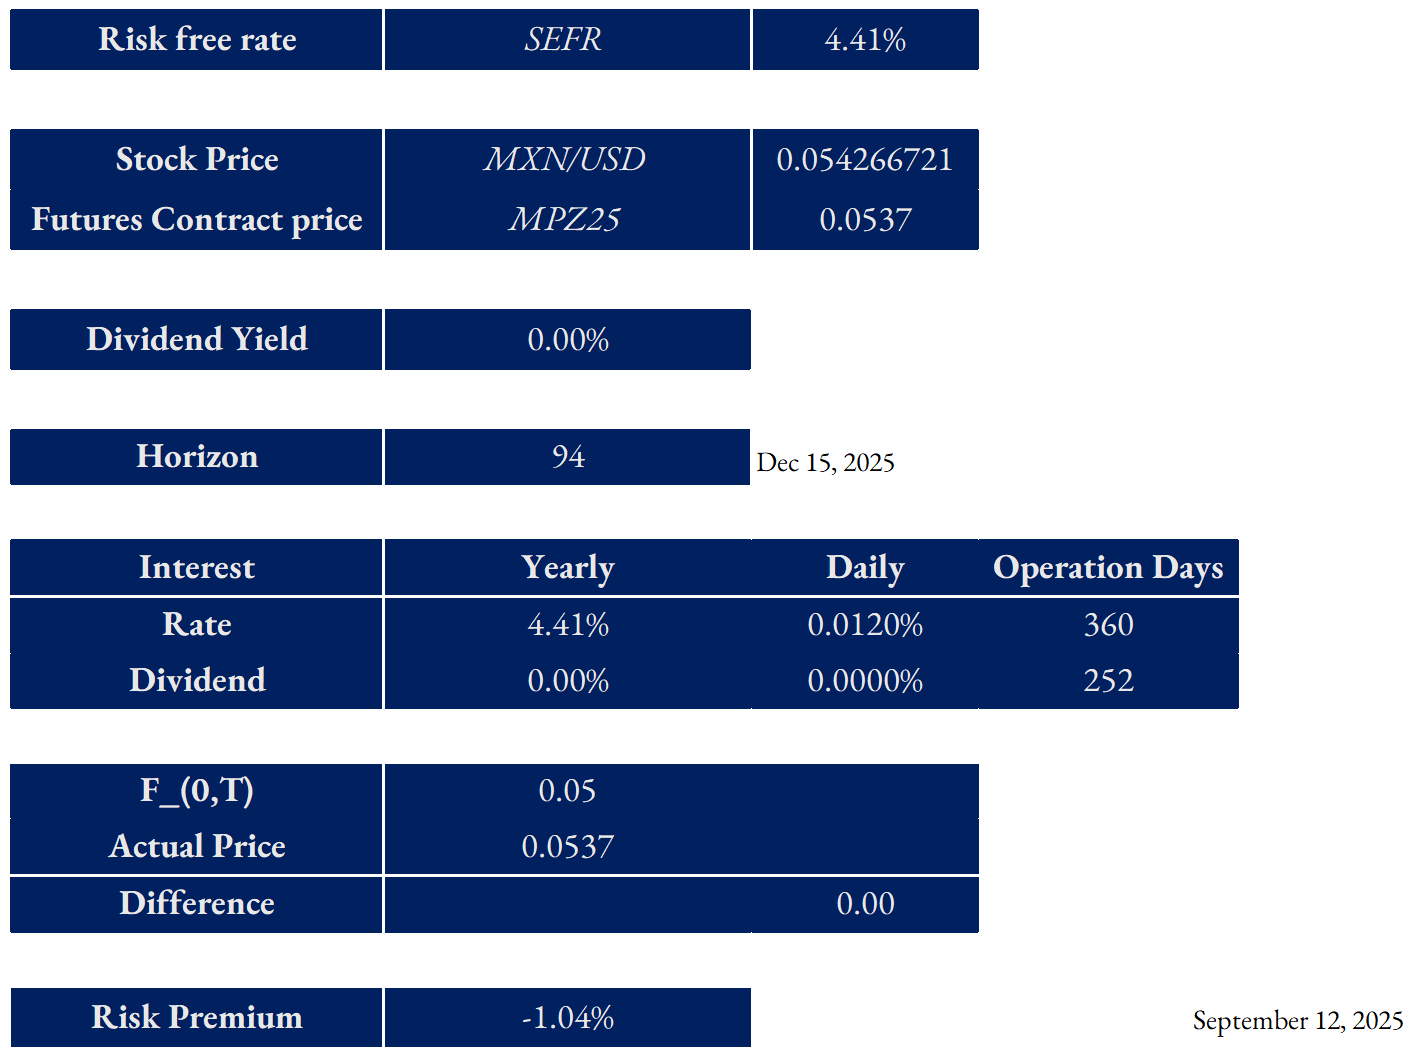
\includegraphics[width=0.7\textwidth]{figures/usdmxn.png}
\caption{Silver price series. Source: Investing.com.}
\end{figure}


\subsubsection{USD/MXN: recent news and pricing implications}

\paragraph{Spot context.}
As of mid-September 2025, USD/MXN trades near 18.45, the peso having reached its strongest levels in over a year amid improved global risk sentiment and lower U.S. rate expectations \citep{reuters_usdmxn_quote,reuters_mx_markets_11sep,reuters_mx_markets_12sep}.

\paragraph{Key developments.}
\begin{enumerate}
  \item \textbf{Federal Reserve path.} A 25 bp cut at the September meeting is widely expected, with markets pricing additional easing by year end; this lowers U.S. rate differentials against MXN and is typically peso-supportive \citep{reuters_fed_poll_2025,reuters_cenbank_graphic_2025}. 
  \item \textbf{Banxico stance and calendar.} Banxico reduced the policy rate to 8.0\% on June 26 and has signaled a gradual path thereafter; the next decision falls on a Thursday at 13:00 CST per the published calendar. A slower easing cadence preserves carry in MXN \citep{reuters_banxico_jun26_2025,banxico_calendar_2025}. 
  \item \textbf{Fiscal guidance.} The draft 2026 budget foresees a narrower deficit (4.1\%/GDP) and includes so-called ``healthy taxes''; improved fiscal optics tend to compress sovereign risk premia and modestly support MXN \citep{reuters_budget_2026_2025}. 
  \item \textbf{Trade policy.} A plan to impose 50\% tariffs on vehicles from non-FTA countries is being advanced; tighter trade measures can weigh on Mexico’s external sector and raise risk premia, which is MXN-negative \citep{reuters_tariffs_autos_2025}. 
  \item \textbf{Pemex credit and sovereign linkages.} A government plan to reduce Pemex debt and a rating upgrade to BB reflect stronger support; improved Pemex credit metrics can narrow Mexico’s risk premium and aid MXN, though execution risk remains \citep{reuters_pemex_plan_2025,reuters_fitch_pemex_2025}. 
\end{enumerate}

\paragraph{Mapping to spot and futures.}
For spot, U.S. rate cuts and steady domestic carry are associated with USD weakness and MXN strength; adverse trade shocks or Pemex slippage work in the opposite direction. For futures, interest-rate parity is used:
\[
F \approx S \, e^{(r_{\mathrm{USD}} - r_{\mathrm{MXN}})T},
\]
so a downward shift in the Fed path (\(r_{\mathrm{USD}}\downarrow\)) is used to lower \(F\) relative to \(S\), while a faster Banxico easing (\(r_{\mathrm{MXN}}\downarrow\)) is used to raise \(F\). Fiscal consolidation and Pemex support compress risk premia that are often embedded in longer-dated forwards, while tariff risks and global-growth shocks are used to widen them \citep{cme_mxn_quotes,cme_fx_overview}.


\paragraph{Measurement.} A small \textbf{positive basis} is observed: the futures price exceeds the theoretical cost-of-carry value by \textbf{20.64 points} $(F=61{,}840 > F^{\*}=61{,}819.36)$, which corresponds to \textbf{0.07\%} on the index. In equity-index pricing, $F^{\*}=S\,e^{(r-q)T}$ is used; therefore a positive $F-F^{\*}$ indicates that the \textbf{market-implied carry} $\hat{c} = \tfrac{1}{T}\ln(F/S)$ is slightly \textbf{above} the model’s $(r-q)$, equivalently that the \textbf{effective dividend drag} expected to expiry is a bit lower than assumed (or that marginal funding is a bit higher).

\paragraph{Interpretation with the news backdrop.} The recent macro mix—Fed easing expectations, supportive global risk appetite, a relatively firm MXN, and locally gradual Banxico guidance—creates a setting in which index futures demand is used to obtain fast beta exposure and dividend-timing risk is perceived as limited. Under these conditions, a \textbf{modestly richer future} vs.\ fair is consistent with: (i) pro-risk positioning that lifts $F$ marginally, (ii) slightly lower expected dividends before expiry, and (iii) liquidity/carry effects as equities trade near highs. The signal is small and lies within typical no-arbitrage frictions; it is read as a \textbf{mild, pro-risk tilt} rather than a standalone mispricing.




\newpage
\section{TIIE}


The TIIE is today the central reference for the cost of overnight peso funding; it is the base price of money used by banks and firms to set interest on loans, bonds, and other instruments. It is estimated with one-day wholesale repo operations settled at INDEVAL, with government or equivalent collateral, and with banks and broker-dealers as participants. Based on these transactions, Banxico reports a representative daily rate and, in addition, \textbf{composition indices} that accumulate daily factors over business or calendar days and ``forward compounded'' versions useful for contracts that require explicit capitalization. The result reflects what actually happened in the market \citep{banxico_methodology,banxico_indices}.

At the CME, the futures contract allows trading the compounded rate; by convention it is quoted as \textbf{Index = 100 - 100R}. For example, today the rate is 8.0126\% and its CME futures price for the TIEU25 contract maturing on September 30, 2025 is 92.28. 

\begin{center}
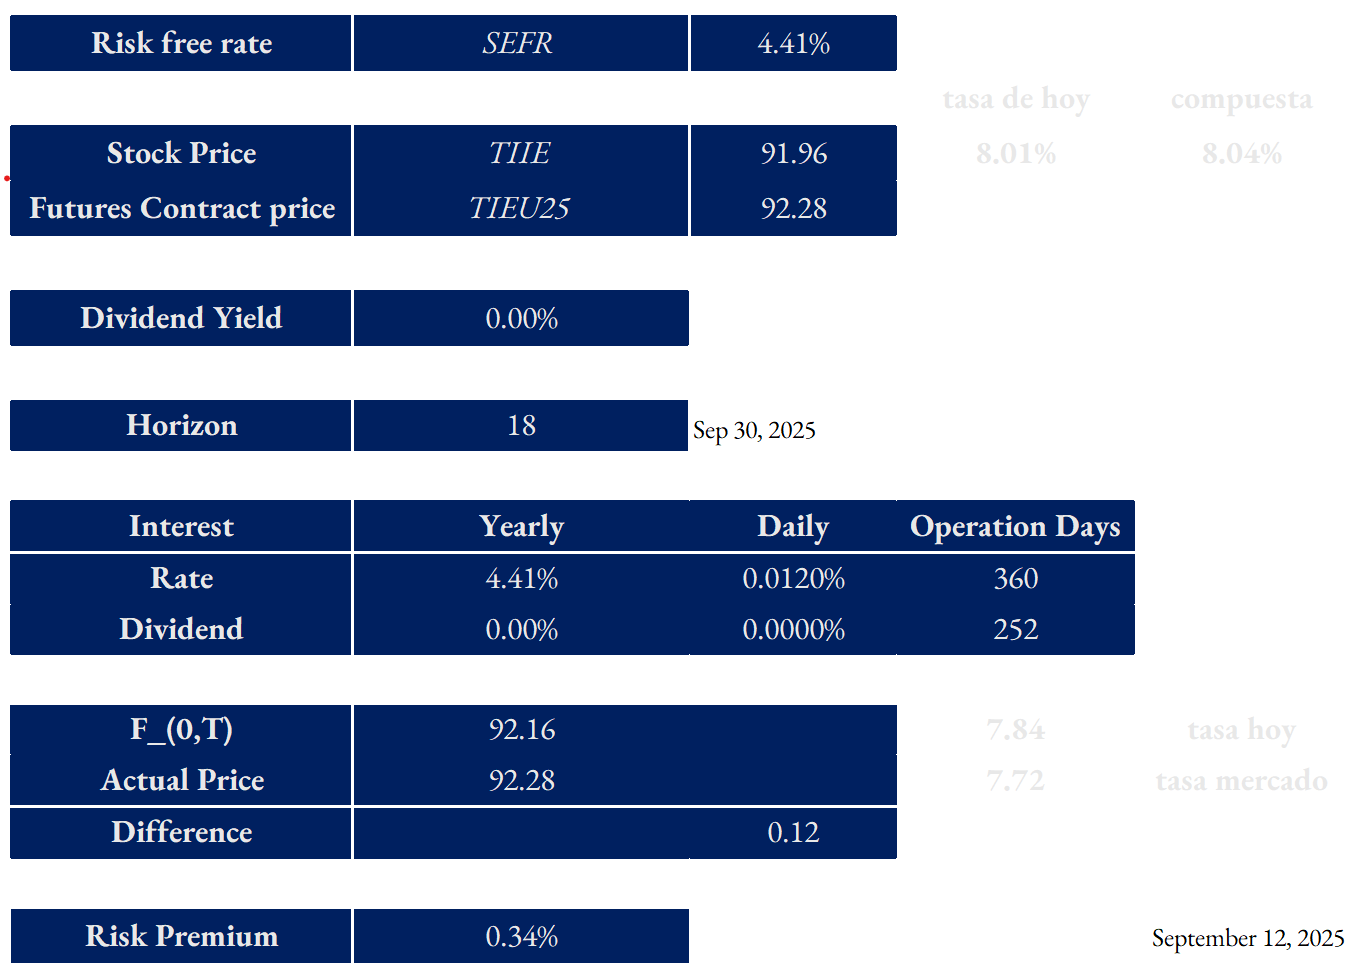
\includegraphics[width=0.5\textwidth]{figures/tiie.png}
\end{center}

A \textbf{positive basis in price} is observed: the \textbf{futures contract} $F=92.28$ is \textbf{above} the theoretical fair value $F^*=92.16$. The \textbf{implied monthly market rate} is therefore about \textbf{12 bps lower} than the model rate, since the market is discounting a \textbf{lower average TIEU25} for the remainder of the month than assumed by the fair value that is, a smoother downward path of rates. In other words, the expectation is for average rates to drift lower. Under the futures convention \textbf{Index = 100 - 100·R}, a \textbf{higher price implies a lower implied rate}. 

From this perspective, the market is effectively pricing a rate of:
\begin{itemize}
  \item \textbf{Market-implied}: $R_{\text{mkt}} = \tfrac{100-92.28}{100} = \mathbf{7.72\%}$.
  \item \textbf{Model (fair)}: $R_{\text{mod}} = \tfrac{100-92.16}{100} = \mathbf{7.84\%}$.
\end{itemize}

\textbf{Current level} (spot TIIE 28d $\approx 8.01\%$): since 12 days have already accrued at $\sim8.01\%$ and 18 days remain, in order for the monthly average to settle at $7.72\%$, the remaining path must evolve near \textbf{7.49\%}. This indicates a market signal of \textbf{gradual softening} of the TIEU25 for the rest of the month.

It is important to emphasize that this reflects an \textbf{expectation of the monthly average}, not a guarantee of an immediate policy cut. The 7.72\% already incorporates carry and the days elapsed; it may be achieved through a steady mild decline or fluctuations around $\sim7.5$--$7.6\%$. If the basis were negative (price $<$ fair), the interpretation would be reversed: an \textbf{implicit rise} in the expected average.

This could be caused by the fact that the Federal Reserve (Fed) is considering rate cuts because the labor market shows signs of cooling, with job creation revised down and unemployment slightly higher, which reduces wage and aggregate demand pressures \citep{reuters2025a}. In addition, inflation, while still above 2\%, shows some moderation and anchored expectations, which allows room for maneuver without eroding credibility \citep{ycharts2025}. At the same time, the policy rate remains in restrictive territory, above neutral, creating the risk of excessive slowdown \citep{ycharts2025}. Moreover, the U.S. economy faces stagnation signals and weaker growth, while the global environment increases vulnerabilities \citep{reuters2025b}. Finally, institutions such as the IMF have noted that the Fed has space to ease its stance given the deterioration in labor dynamics \citep{reuters2025c}, and Powell himself has acknowledged employment risks as an argument to open the door to cuts \citep{reuters2025d}.

If the Fed starts cutting and the peso remains stable, the market usually anticipates that the rate $R$ will decline; then the TIIE futures price rises. The approximate profit or loss per contract is 
\[
\Delta \text{P\&L} \approx 50{,}000 \times \Delta \text{Index} \quad \text{MXN}
\]
\citep{banxico2023,cme2025a,cme2025b,reuters2025a}. 

The process can be described as follows:

\begin{enumerate}
    \item New information arrives. For example, lower inflation signals in the U.S. and Fed guidance toward \textbf{consecutive cuts} \citep{reuters2025}.
    \item Very short-term USD rates fall. Dollar funding becomes cheaper and the expected path shifts downward.
    \item Global financial conditions ease. Lower risk aversion and often a weaker USD reduce imported inflationary pressure in Mexico.
    \item Banxico assesses the local picture. If inflation and the exchange rate cooperate, the market anticipates local cuts with a \textbf{lag} relative to the Fed. That \textbf{expected path} is what matters for derivatives.
    \item The expected TIEU25 for the quarter decreases. The compounded TIEU25 of the period, $R$, falls if each daily ``drop'' is slightly smaller.
    \item The futures price rises. By convention, \textbf{lower $R \Rightarrow$ higher Index}, because Index $= 100 - R$. A change of $-25$ bp in $R$ implies $+\!0.25$ index points.
\end{enumerate}

As an example, suppose the market expects an annualized compounded rate of $R = 10.00\%$. The futures contract trades near $100 - 10.00 = 90.00$. If, after cut guidance, consensus shifts to $R = 9.75\%$, the price would be 90.25. The approximate variation for a long contract is:

\[
\Delta \text{P\&L} \approx (90.25 - 90.00)\times 50{,}000 = \textbf{12{,}500 \ \text{MXN}}.
\]

Of course, this is not always the case, for several reasons:

\begin{itemize}
    \item \textbf{Local decoupling.} A rebound in Mexican inflation or a peso depreciation may lead Banxico to delay or cut less; $R$ falls less and the futures price rises less or corrects.
    \item \textbf{Technical factors.} Term premiums, paper supply, repositioning, or calendar effects. The compounding methodology extends the last published rate on weekends and holidays, introducing small differences across months and quarters and a \textbf{basis} between what you want to hedge and what the contract settles \citep{cme2025a,cme2025b}.
\end{itemize}



\section{IPC}

The S\&P/BMV IPC is the flagship index of the Mexican equity market, designed to measure the performance of the largest and most liquid stocks listed on the Bolsa Mexicana de Valores (BMV). It is float-adjusted, market-cap weighted, and maintained under published rules with regular rebalances \citep{spdj_ipc_page,spdj_bmv_methodology}.

\paragraph{Derivatives and implementation.}
Exposure and hedging are available via IPC futures listed at MexDer; these contracts are designed to manage equity-market risk tied to the Mexican market benchmark \citep{mexder_ipc_fut}.

\paragraph{Nowcasting the next move: macro–market linkages.}
As of \emph{September 12, 2025}, the IPC printed a new all-time high near 61{,}900, supported by risk-on flows as markets price imminent Fed cuts; the peso hovered around 18.4 per USD \citep{reuters_ipc_record_2025,reuters_usdmxn_quote}. This backdrop interacts with Mexico’s local cycle and policy mix:

\begin{enumerate}
    \item \textbf{Fed trajectory and global risk appetite.} Rising odds of a September Fed cut lowered U.S. yields and improved EM risk sentiment, historically supportive for Mexico’s equities and currency \citep{reuters_ipc_record_2025}.
    \item \textbf{Banxico path and inflation.} Recent data show headline inflation ticking up, prompting a slower easing cadence even as inflation expectations remain near target; net effect: supportive discount-rate impulse, but gradual \citep{bloomberg_mx_inflation_2025,mnd_inflation_band_2025}.
    \item \textbf{Fiscal stance and sovereign risk.} The 2026 budget narrative points to a slightly narrower deficit after 2025, with attention on execution and quasi-sovereign exposures (e.g., Pemex) that shape risk premia and equity multiples \citep{reuters_budget_2025,reuters_pemex_plan_2025}.
    \item \textbf{Trade/industrial policy shocks.} Proposed 50\% tariffs on vehicles from non-FTA countries would rewire EV/auto pricing in Mexico, with potential rotation across consumer, industrial, and materials names via supply-chain and price-elasticity channels \citep{reuters_tariffs_china_autos_2025}.
    \item \textbf{Nearshoring vs.\ frictions.} The medium-term nearshoring thesis coexists with cyclical frictions; recent reports of border-maquiladora job losses tied to U.S. tariff dynamics illustrate downside risk to industrial earnings momentum \citep{reuters_border_jobs_2025}.
\end{enumerate}

\paragraph{Base case and risks.}
Netting these forces, the near-term base case is a \emph{carry-and-liquidity-supported drift} while the Fed turns, tempered by Banxico’s gradualism and policy noise. Upside risks: faster global disinflation and credible domestic fiscal/Pemex execution that compress risk premia. Downside risks: renewed inflation pressure, sharper USD strength, escalation of tariff frictions, or disappointing growth that erodes earnings leverage \citep{reuters_ipc_record_2025,bloomberg_mx_inflation_2025,reuters_budget_2025,reuters_pemex_plan_2025,reuters_tariffs_china_autos_2025}.

\begin{figure}[h]
\centering
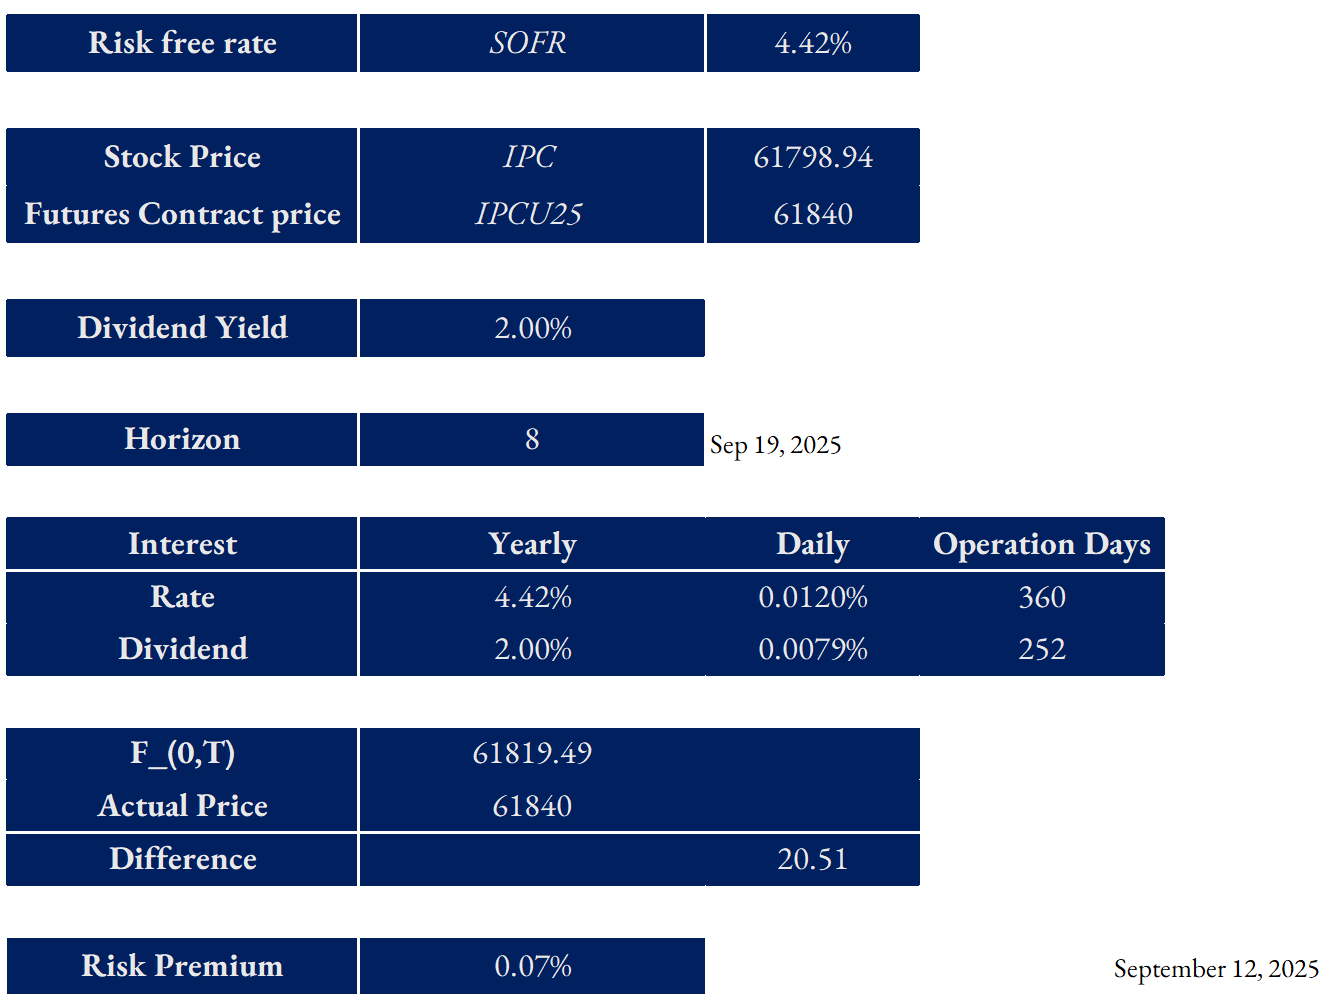
\includegraphics[width=0.7\textwidth]{figures/ipc.png}
\caption{Silver price series. Source: Investing.com.}
\end{figure}

\paragraph{Measurement.} A small \textbf{positive basis} is observed: the futures price exceeds the theoretical value by \textbf{20.64 points} $(F=61{,}840 > F^{*}=61{,}819.36)$. In equity-index futures priced via the cost-of-carry relation $F^{*}=S\,e^{(r-q)T}$, a positive $F-F^{*}$ is interpreted as a market-implied carry $\hat{c} = \tfrac{1}{T}\ln(F/S)$ that is \textbf{slightly above} the model’s $(r-q)$. Equivalently, the market is embedding a \textbf{lower effective dividend yield} over the remaining horizon (or marginally higher funding) than the one used in the model. Expressed on the underlying, the premium equals \textbf{$\approx 0.07\%$}, which is economically small and typically falls within no-arbitrage frictions (bid–ask, financing haircuts, dividend-timing uncertainty, and LAST vs SETTLE timing).

\paragraph{Interpretation with the news background.} In a setting where risk appetite is supported by anticipated Fed easing, a firm MXN, and benign local discount-rate dynamics, a \textbf{slightly richer future} is consistent with: (i) \textbf{long-demand in futures} to gain rapid benchmark exposure, (ii) \textbf{temporarily lower dividend-drag} expected between now and expiry, and (iii) \textbf{carry-and-liquidity effects} when equity rallies compress index lending spreads. The signal is therefore read as a \textbf{modest, pro-risk tilt}—not a standalone arbitrage—indicating that the market prices a marginally easier near-term environment for Mexican equities than implied by the model inputs.




\section{Bibliography}
\bibliography{refs}



\end{document}